\documentclass[12pt, a4paper]{report}
\usepackage[utf8]{vietnam}
\usepackage{array, makecell}
\usepackage{graphicx, graphics}
\renewcommand\theadfont{\bfseries}
\usepackage{tikz}
\usepackage{xcolor}
\usepackage{wrapfig}
\usepackage{multicol}
\usepackage{indentfirst}
\usepackage{fancybox}%dùng gói fancybox tự tìm trên mạng nha
\usepackage[left=3cm, right=3cm, top=3cm, bottom=3cm]{geometry}
\usepackage{fancyhdr}
\pagestyle{fancy}
\fancyhf{}
% \rhead{Đồ án II}
\lhead{Báo cáo Đồ án II}
\renewcommand{\footrulewidth}{0.5pt}
\lfoot{Nguyễn Văn Triển - 20195934}

\begin{document}
\begin{titlepage}
	\thispagestyle{empty}
%\thisfancypage{%đóng khung trang này
%\setlength{\fboxsep}{0pt}% 8pt là độ dày của đường viền
%\fbox}{} % phần nội dung sau là tương tự như đã làm
    \begin{tikzpicture}[remember picture,overlay,inner sep=0,outer sep=0]
      \draw[blue!70!black,line width=5pt] 
      ([xshift=-2cm,yshift=-2cm]current page.north east) coordinate (A)--
      ([xshift=2cm,yshift=-2cm]current page.north west) coordinate(B)--
      ([xshift=2cm,yshift=2cm]current page.south west) coordinate (C)--
      ([xshift=-2cm,yshift=2cm]current page.south east) coordinate(D)--cycle;

      \draw ([yshift=0.5cm,xshift=-0.5cm]A)-- ([yshift=0.5cm,xshift=0.5cm]B)--
      ([yshift=-0.5cm,xshift=0.5cm]B) --([yshift=-0.5cm,xshift=-0.5cm]B)--([yshift=0.5cm,xshift=-0.5cm]C)--([yshift=0.5cm,xshift=0.5cm]C)--([yshift=-0.5cm,xshift=0.5cm]C)-- ([yshift=-0.5cm,xshift=-0.5cm]D)--([yshift=0.5cm,xshift=-0.5cm]D)--([yshift=0.5cm,xshift=0.5cm]D)--([yshift=-0.5cm,xshift=0.5cm]A)--([yshift=-0.5cm,xshift=-0.5cm]A)--([yshift=0.5cm,xshift=-0.5cm]A);


      \draw ([yshift=-0.3cm,xshift=0.3cm]A)-- ([yshift=-0.3cm,xshift=-0.3cm]B)--
      ([yshift=0.3cm,xshift=-0.3cm]B) --([yshift=0.3cm,xshift=0.3cm]B)--([yshift=-0.3cm,xshift=0.3cm]C)--([yshift=-0.3cm,xshift=-0.3cm]C)--([yshift=0.3cm,xshift=-0.3cm]C)-- ([yshift=0.3cm,xshift=0.3cm]D)--([yshift=-0.3cm,xshift=0.3cm]D)--([yshift=-0.3cm,xshift=-0.3cm]D)--([yshift=0.3cm,xshift=-0.3cm]A)--([yshift=0.3cm,xshift=0.3cm]A)--([yshift=-0.3cm,xshift=0.3cm]A);

    \end{tikzpicture}
    
\begin{center}
    %\textbf{ }\\[10pt]
    \textbf{
    \begin{LARGE}
    ĐẠI HỌC BÁCH KHOA HÀ NỘI
    \end{LARGE} \\
    \begin{large}
    VIỆN TOÁN ỨNG DỤNG VÀ TIN HỌC
    \end{large} 
    }\\[12pt]
    \textbf{--------------------  *  ---------------------}\\[5pt]
    
\includegraphics[scale=0.8]{./image/logo.jpg}\\[12pt]
    {\fontsize{18pt}{1}\selectfont BÁO CÁO ĐỒ ÁN II}\\[1.5cm]
    {\fontsize{18pt}{1}\selectfont Đề tài: Phân tích, thiết kế hệ thống web quản lý học tập và đăng ký đồ án, thực tập của sinh viên}\\[12pt]

    \textbf{ }\\
    
  \end{center}
  \begin{tabular}{lllll}
      Giảng viên hướng dẫn&: & \textbf{TS. Ngô Quốc Hoàn} &&\\
      Sinh viên thực hiện&: & Nguyễn Văn Triển &&\\
      MSSV&: & 20195934 &&\\
      % Lớp: & Toán tin 02 - K64 & $\overline{\text{Chữ ký của GVHĐ}}$
      Lớp&: & Toán tin 02 - K64 && \textoverline{Chữ ký của GVHD}
      % \fontsize{16pt}{30}{$\overline{\text{Chữ ký của GVHD}}$}
  \end{tabular}\\
  % \hspace{4pt}\textbf{Chữ}
\vspace{2.5cm}
\begin{center}
{\fontsize{14pt}{1}\selectfont Hà Nội, tháng 03 năm 2023}
\end{center}

	\newpage
\thispagestyle{empty}
%nhận xét của giảng viên
\begin{center}
    NHẬN XÉT CỦA GIẢNG VIÊN
\end{center}
\textbf{1. Mục đích và nội dung đồ án}
\begin{itemize}
    \item[-] \textbf{Mục đích}: 
    \vspace{2cm}
    \item[-] \textbf{Nội dung}: 
    \vspace{2cm}

\end{itemize}
\textbf{2. Kết quả đạt được}
\begin{itemize}
    \item[-] 
    \item[-] 
    \item[-] 
    \item[-] 
    
\end{itemize}
\textbf{3. Ý thức làm việc của sinh viên}
\begin{itemize}
    \item[-] 
\end{itemize}
\vspace{3cm}
\vspace{.5cm}
\hspace{0.5\textwidth}
\begin{minipage}{0.5\textwidth}
	\noindent\begin{center}
% 		\vspace{1cm}
		\textit{Hà Nội, ... tháng 3 năm 2023} \\
		Giảng viên hướng dẫn\\ \vspace{2cm}
		\textbf{TS. Ngô Quốc Hoàn} \\
	\end{center}	
\end{minipage}

	\newpage
\pagenumbering{gobble}
\chapter*{Lời cảm ơn}
    Lời đầu tiên em xin được bày tỏ lòng biết ơn sâu sắc đến các thầy cô Viện Toán ứng dụng và Tin học, Đại học Bách Khoa Hà Nội đã truyền đạt những kiến thức nền tảng hữu ích xuyên suốt các kỳ học qua để từ đó giúp em có những kiến thức và kĩ năng tốt hơn trong quá trình tìm hiểu và nghiên cứu đề tài.
    
    Đặc biệt em xin bày tỏ lòng biết ơn chân thành sâu sắc tới \textbf{TS. Ngô Quốc Hoàn} đã trực tiếp giúp đỡ, hướng dẫn em hoàn thành Đồ án 2 này. Thầy đã dành nhiều thời gian hướng dẫn, chia sẻ những kiến thức, tài liệu hay và đưa ra các hướng dẫn cải tiến Đồ án từ nội dung tới cách trình bày để giúp bài báo cáo của em được tốt nhất.
    
    Em cũng chân thành cảm ơn những chia sẻ góp ý quý báu của \textbf{TS. Lê Chí Ngọc} trong quá trình em thực hiện đồ án. 
		Những ý kiến đóng góp của thầy cô sẽ giúp em nhận ra những hạn chế và qua đó em có thêm những kiến thức, nguồn tư liệu mới trên con đường học tập cũng như nghiên cứu sau này.
    
    Em xin chân thành cảm ơn!
    
\vspace{1.5cm}
\hspace{0.5\textwidth}
\begin{minipage}{0.5\textwidth}
	\noindent\begin{center}
% 		\vspace{1cm}
		\textit{Hà Nội, ... tháng 3 năm 2023} \\
		Sinh viên\\ \vspace{2cm}
		\textbf{Nguyễn Văn Triển} \\
	\end{center}	
\end{minipage}
\newpage
	\newpage
	\tableofcontents
\end{titlepage}
\newpage
\setcounter{page}{1}
\pagenumbering{arabic}
\rfoot{\thepage}

\chapter*{Mở đầu}
\chapter{Tổng quan về đề tài}
\section{Lý do chọn đề tài}
Mỗi năm, Đại học Bách khoa Hà Nội tuyển sinh khoảng 8000 sinh viên (theo số liệu 2022). 
Để thực hiện tốt việc hỗ trợ sinh viên một cách đầy đủ nhất, công tác quản lý sinh viên (kết quả học tập của sinh viên) đóng vai trò hết sức quan trọng đối với hoạt động của một khoa/viện trong các trường đại học.

Quản lí các dữ liệu có thể biết được những sinh viên đang chậm tiến độ học tập, những sinh viên đang bị mức cảnh cáo học tập để từ đó đưa ra giải pháp, tư vấn học tập phù hợp đối với các sinh viên.
Ngoài ra, hiện nay các vấn đề về đăng ký làm đồ án, đăng ký thực tập cho sinh viên đang được diễn ra một cách thủ công dưới hình thức điền form truyền thống.
Điều đó dẫn tới tốn rất nhiều thời gian để giảng viên sắp xếp, phản hồi, ... 
Hệ thống chủ yếu hướng tới người dùng là những sinh viên năm cuối sắp ra trường, từ đó tạo điều kiện tốt nhất để mang đến những định hướng đúng đắn, phù hợp cho sinh viên.
Ngoài ra, khi ra trường các sinh viên có thể kết nối thông tin đến với các doanh nghiệp một cách dễ dàng hơn.
Sự đồng hành của thầy cô, đặc biệt là giảng viên chuyên ngành - những người gần gũi, có thể phát hiện ra vấn đề của các sinh viên đó là rất quan trọng.
Hệ thống sẽ giúp các khoa/viện định hướng nghề, hỗ trợ kỹ năng tìm việc cho sinh viên để mọi người chuẩn bị tốt hơn cho tương lai.
Bên cạnh đó, hệ thống cũng giúp sinh viên dễ dàng hơn trong quá trình tìm hiểu cũng như chọn đề tài đồ án, vị trí thực tập của mình.

\subsection*{Khảo sát hệ thống}

\noindent Đánh giá kết quả học tập của Đại học Bách khoa Hà Nội:\textsuperscript{\cite{daotao}}
\begin{itemize}
	\item[1.] Kết quả học tập trong một học kỳ của sinh viên được đánh giá trên cơ sở điểm của các học phần thuộc chương trình đào tạo không kể các học phần có điểm R (điểm học phần được miễn học và công nhận tín chỉ) và các môn yêu cầu chứng chỉ riêng (Ngoại ngữ, Giáo dục thể chất, Giáo dục quốc phòng-an ninh), thể hiện bằng các chỉ số:
		\begin{itemize}
			\item[a.] Số tín chỉ đạt là tổng số tín chỉ của các học phần có điểm đạt trong học kỳ.
			\item[b.] Số tín chỉ không đạt là tổng số tín chỉ của các học phần có điểm không đạt trong học kỳ.
			\item[c.] Điểm trung bình học kỳ (GPA) là trung bình cộng điểm số quy đổi theo thang 4 của các học phần mà sinh viên đã học trong học kỳ với trọng số là số tín chỉ của học phần. Điểm trung bình học kỳ được làm tròn tới 2 chữ số thập phân.
		\end{itemize}
	\item[2.] Kết quả tiến bộ học tập của sinh viên từ đầu khoá được đánh giá trên cơ sở điểm của các học phần thuộc chương trình đào tạo không kể các môn yêu cầu chứng chỉ riêng, thể hiện bằng các chỉ số:
		\begin{itemize}
			\item[a.] Số tín chỉ tích luỹ (TCTL) là tổng số tín chỉ của các học phần đã đạt từ đầu khoá kể cả các học phần được miễn, được chuyển điểm.
			\item[b.] Số tỉn chỉ nợ tồn đọng là tổng số tín chỉ của các học phần đã học nhưng chưa đạt từ đầu khoá.
			\item[c.] Điểm trung bình tích luỹ (CPA) là trung bình cộng điểm số quy đổi theo thang 4 của các học phần đã học từ đầu khoá với trọng số là số tín chỉ của học phần. Điểm trung bình tích luỹ được làm tròn tới 2 chữ số thập phân.
			\item[d.] Trình độ ngoại ngữ của sinh viên đạt được theo yêu cầu chương trình đào tạo, thể hiện qua kết quả thi nội bộ trong trường và các chứng chỉ ngoại ngữ được xét tương đương.
		\end{itemize}
	\item[3.] Sinh viên được xếp hạng trình độ năm học căn cứ số tín chỉ tích luỹ như sau:
    \begin{table}[h!]
      \begin{tabular}{|l|c|c|c|c|c|}
          \hline
          Số TCTL  & $<32$        & $32-63$     & $64-95$    & $96-127$   & $\geq 128$  \\
          \hline
          Trình độ & Năm thứ nhất & Năm thứ hai & Năm thứ ba & Năm thứ tư & Năm thứ năm \\
          \hline
        \end{tabular}   
    \end{table}	
	\item[4.] Sinh viên được xếp loại học lực theo học kỳ căn cứ điểm trung bình học kỳ và xếp loại học lực từ đầu khoá căn cứ điểm trung bình tích luỹ như sau:
    \begin{table}[h!]
      \begin{tabular}{|l|c|c|c|c|c|c|c|}
          \hline
          GPA/CPA  & $<1.0$ & $1.0-1.49$ & $1.5-1.99$ & $2.0-2.49$ & $2.5-3.19$ & $3.2-3.59$ & $3.6-4.0$ \\
          \hline
          Xếp loại & Kém    & Yếu        & TB yếu     & Trung bình & Khá        & Giỏi       & Xuất sắc  \\
          \hline
        \end{tabular}
    \end{table}	
\end{itemize}

\noindent Xử lý kết quả học tập Đại học Bách Khoa Hà Nội:\textsuperscript{\cite{daotao}}\\

Các hình thức xử lý kết quả học tập được áp dụng cuối mỗi học kỳ chính, bao gồm cảnh cáo học tập (mức 1 đến mức 3), buộc thôi học và hạn chế khối lượng đăng ký học tập.
\begin{itemize}
  \item[1.] Cảnh cáo học tập là hình thức cảnh cáo những sinh viên có kết quả học tập yếu kém, áp dụng cụ thể như sau:
    \begin{itemize}
      \item[a.] Nâng một mức cảnh cáo đối với sinh viên có số tín chỉ không đạt trong học kỳ lớn hơn 8.
      \item[b.] Nâng hai mức cảnh cáo đối với sinh viên có số tín chỉ không đạt trong học kỳ lớn hơn 16 hoặc tự ý bỏ học, không đăng ký học tập. 
      \item[c.] Áp dụng cảnh cáo mức 3 đối với sinh viên có số tín chỉ nợ tồn đọng từ đầu khoá lớn hơn 27.
      \item[d.] Sinh viên đang bị cảnh cáo học tập, nếu số tín chỉ không đạt trong học kỳ bằng hoặc nhỏ hơn 4 thì được hạ một mức cảnh cáo.  
    \end{itemize}
  \item[2.] Buộc thôi học là hình thức áp dụng đối với những sinh viên có kết quả quá trình học tập rất kém, cụ thể trong các trường hợp như sau:
    \begin{itemize}
      \item[a.] Sinh viên bị cảnh cáo học tập mức 3, ngoại trừ những đối tượng được hưởng chế độ ưu tiên trong đào tạo theo quy định của Bộ thì được nộp đơn xin gia hạn một học kỳ và chỉ một lần trong toàn khoá học.
      \item[b.] Sinh viên học vượt quá thời gian cho phép, hoặc không còn đủ khả năng tốt nghiệp trong thời gian cho phép theo quy định tại Điều 6.
    \end{itemize}
  \item[3.] Hạn chế khối lượng học tập là hình thức buộc những sinh viên học yếu kém hoặc chưa đạt chuẩn ngoại ngữ (xét tại thời điểm đăng ký học tập) đăng ký số tín chỉ học phần chuyên môn ít hơn bình thường, cụ thể như sau:
    \begin{itemize}
      \item[a.] Sinh viên bị cảnh cáo học tập mức 1 được đăng ký tối đa 18 TC và tối thiểu 10 TC cho một học kỳ chính.
      \item[b.] Sinh viên bị cảnh cáo học tập mức 2 được đăng ký tối đa 14 TC và tối thiểu 8 TC cho một học kỳ chính.
      \item[c.] Sinh viên không đạt chuẩn ngoại ngữ theo quy định cho từng trình độ năm học được đăng ký tối đa 14 TC và tối thiểu 8 TC cho một học kỳ chính.  
    \end{itemize}
\end{itemize}

\subsubsection*{Quản lý hồ sơ sinh viên}
	Hồ sơ sinh viên là một phần thiết yếu của việc quản lý sinh viên trong các hệ thống Đại học. 
	Chúng chứa thông tin quan trọng về các sinh viên như thông tin cá nhân, tiến độ học tập, ... 
	Quản lý hồ sơ sinh viên một cách hiệu quả là rất quan trọng để đảm bảo rằng sinh viên nhận được sự hỗ trợ cần thiết để thành công trong học tập và cá nhân.

	Khi các cán bộ giảng viên muốn biết thông tin về sinh viên nào đó thì có thể sử dụng hồ sơ mà chúng ta quản lý để tìm thông tin về họ.
	Từ đó nắm thông tin một cách nhanh chóng cũng như chính xác nhất. 
\subsubsection*{Quản lý học tập sinh viên}
	Quản lý học tập của sinh viên đề cập đến việc tiếp cận có hệ thống để quản lý quá trình học tập cho sinh viên. 
	Điều này bao gồm mọi thứ từ thiết kế và cung cấp nội dung giáo dục đến theo dõi sự tiến bộ của sinh viên và cung cấp hỗ trợ khi cần thiết.
	Một hệ thống quản lý học tập cho phép giảng viên tạo và chia sẻ nội dung giáo dục hấp dẫn, theo dõi hiệu suất của sinh viên, cung cấp phản hồi kịp thời và xác định các lĩnh vực cần hỗ trợ thêm.
	Mục tiêu cuối cùng của quản lý học tập của sinh viên là đảm bảo rằng sinh viên đang nhận được một nền giáo dục chất lượng để chuẩn bị cho họ thành công trong tương lai.
	Quản lý học tập hiệu quả đòi hỏi sự kết hợp giữa công nghệ, phương pháp sư phạm và quá trình ra quyết định dựa trên dữ liệu để tạo ra một môi trường học tập tối ưu cho sinh viên.
\subsubsection*{Quản lý đăng ký đồ án của sinh viên}
	Việc quản lý đăng ký đồ án của sinh viên là một khía cạnh thiết yếu của quản lý sinh viên trong hệ thống Đại học. Nó liên quan đến việc thiết lập một hệ thống nơi sinh viên có thể đăng ký đồ án của họ và nhận hỗ trợ trong suốt thời gian của dự án.
	Đăng ký đồ án giúp đảm bảo rằng sinh viên đang thực hiện các dự án có liên quan và có ý nghĩa, phù hợp với sở thích và mục tiêu học tập của họ. 
	Một hệ thống đăng ký dự án tốt sẽ cho phép dễ dàng đăng ký và theo dõi các đồ án, cũng như cung cấp cho sinh viên quyền truy cập vào các tài nguyên, cố vấn và phản hồi.
	Quản lý hiệu quả đăng ký đồ án của sinh viên đòi hỏi sự kết hợp của các hướng dẫn rõ ràng, thông tin liên lạc minh bạch và hỗ trợ từ giảng viên. 
	Bằng cách triển khai một hệ thống đăng ký đồ án mạnh mẽ, các tổ chức giáo dục có thể thúc đẩy văn hoá đổi mới, sáng tạo và hợp tác giữa các sinh viên.
\subsubsection*{Quản lý đăng ký thực tập của sinh viên}
	Cũng như quản lý đồ án, quản lý đăng ký thực tập của sinh viên là một nội dung quan trọng của công tác quản lý sinh viên nhất là đối với các sinh viên năm cuối.
	Thực tập mang lại cơ hội quý giá cho sinh viên để có được kinh nghiệm thực tế trong lĩnh vực nghiên cứu của họ và tạo mối quan hệ với các chuyên gia trong ngành mà họ đã chọn.
	Quản lý đăng ký thực tập liên quan đến việc thiết lập một hệ thống nơi sinh viên có thể dễ dàng tìm và đăng ký thực tập phù hợp với sở thích và mục tiêu học tập của họ.
	Nó cũng liên quan đến việc đảm bảo rằng sinh viên nhận được sự hỗ trợ mà họ cần trong suốt quá trình thực tập, chẳng hạn như đăng ký thường xuyên, hướng dẫn hoàn thành nhiệm vụ và cơ hội nhận phản hồi.
	Một hệ thống đăng ký thực tập tốt phải minh bạch, hiệu quả và cung cấp cho sinh viên khả năng tiếp cận nhiều cơ hội thực tập.
	Quản lý hiệu quả việc đăng ký thực tập của sinh viên đòi hỏi sự hợp tác chặt chẽ giữa giảng viên, doanh nghiệp và các đối tác trong ngành để đảm bảo rằng sinh viên có được kinh nghiệm quý báu và phát triển các kỹ năng cần thiết để thành công trong sự nghiệp đã chọn.

\subsubsection*{Nhược điểm của phương pháp quản lý truyền thống hiện nay}
	Việc quản lý thủ công thông tin và hồ sơ của sinh viên là một quá trình tốn nhiều thời gian và rườm rà. 
	Không những thế việc đó có thể dẫn đến sai sót trong quá trình nhập, xử lý và truy xuất dữ liệu.
	Có thể khó duy trì tính chính xác và nhất quán của hồ sơ khi xử lý khối lượng lớn dữ liệu theo cách thủ công.

	Hiện nay, hệ thống quản lý sinh viên của Đại học Bách khoa Hà Nội đã được số hoá, tuy nhiên vẫn còn một số hạn chế chẳng hạn, 
	khó theo dõi được tình hình học tập, mức độ cảnh cáo của các sinh viên.
	Việc đăng ký đồ án, thực tập vẫn được thực hiện một cách thủ công thông qua điền form trực tuyến và sau đó cán bộ sẽ sắp xếp, trả kết quả lại cho sinh viên.
	Việc tiếp cận các thông tin về đề tài đồ án, thông tin thực tập của sinh viên còn nhiều hạn chế.

\section{Yêu cầu của bài toán}
%sửa
Xuất phát từ nhu cầu đổi mới và phù hợp với sự phát triển của xã hội ngày nay, việc thay đổi hệ thống quản lý cũ bằng một hệ thống quản lý mới tối ưu hơn là một điều tất yếu.

Hệ thống mới cho phép quản lý 10000 người dùng bao gồm sinh viên, giảng viên, cán bộ và người quản trị hệ thống.
Hệ thống giúp rút ngắn thời gian đăng ký cũng như chờ đợi của sinh viên. Việc lưu trữ cũng trở nên đơn giản, không cần phải có nơi lưu trữ lớn, các thông tin về sinh viên sẽ chính xác và nhanh chóng.

Mỗi sinh viên sẽ sử dụng tài khoản microsoft mail trường cấp của mình để đăng ký tài khoản người dùng, sau đó có thể liên kết với
các tài khoản xã hội khác (google gmail, facebook). 
Hệ thống quản lý sinh viên bao gồm các chức năng:
\begin{itemize}
	\item Đăng ký, đăng nhập, đăng xuất khỏi hệ thống.
	\item Cập nhật thông tin cá nhân (điểm học tập).
	\item Tra cứu thông tin đề tài đồ án, giảng viên hướng dẫn.
	\item Tra cứu thông tin công ty thực tập.
	\item Đăng ký đồ án.
	\item Tạo CV cá nhân dành cho sinh viên.
	\item Đăng ký thực tập.
	\item Thống kê kết quả học tập của sinh viên dành cho giảng viên.
\end{itemize}

\section{Tác nhân của hệ thống}
\begin{tabular}{|c|c|l|}
	\hline
	\thead{STT} & \thead{Tác nhân} & \thead{Chức năng}                                                        \\
	\hline
	1           & Quản trị viên    & \makecell[l]{- Quản trị hệ thống.                                        \\ - Phân quyền người dùng. \\ - Cấp lại mật khẩu cho người dùng.}\\
	\hline
	2           & Cán bộ           & \makecell[l]{- Quản lý danh sách sinh viên.                              \\ - Quản lý form đăng ký trả về.} \\
	\hline
	3           & Giảng viên       & \makecell[l]{- Quản lý danh sách sinh viên theo lớp.}                         \\
	\hline
	4           & Sinh viên        & \makecell[l]{- Đăng nhập, đăng ký, đăng xuất, cập nhật thông tin.        \\ - Sử dụng hệ thống, thực hiện điền form. \\ - Tìm kiếm, tra cứu thông tin.}\\
	\hline
\end{tabular}

\section{Mô tả hệ thống}
\subsection{Dành cho quản trị viên}
\begin{itemize}
	\item Đăng nhập, đăng xuất khỏi hệ thống
	\item Phân quyền người dùng, quản trị hệ thống
\end{itemize}
\subsection{Dành cho sinh viên}
\begin{itemize}
	\item Mỗi sinh viên có thể sử dụng tài khoản Microsoft do nhà trường cung cấp (đuôi @sis.hust.edu.vn hoặc @hust.edu.vn) để đăng ký tài khoản sau đó liên kết với các tài khoản khác (Google, Facebook, ...). Sau đó có thể sử dụng một trong các tài khoản này để đăng nhập vào hệ thống. Khi đăng nhập thành công sẽ hiển thị giao diện trang chủ.
	\item Sinh viên có thể cập nhật thông tin cá nhân (tên, lớp, trạng thái học tập, điểm CPA, số tín chỉ đã qua, số tín chỉ nợ, ...) tại trang cá nhân.
	\item Sinh viên có thể tìm kiếm thông tin về đề tài đồ án (đồ án I, đồ án II, đồ án tốt nghiệp), thông tin giảng viên hướng dẫn.
	\item Sinh viên có thể thực hiện nhập thông tin đăng ký đồ án, xem trạng thái đăng ký, chờ kết quả trả về.
	\item Sinh viên có thể tìm kiếm các thông tin thực tập: vị trí, công ty, lĩnh vực.
	\item Sinh viên có thể thực hiện điền các thông tin cá nhân khác (giới thiệu bản thân, kinh nghiệm, các dự án tham gia, ...) để từ đó hệ thống sẽ lưu dữ liệu và xuất ra bản CV để từ đó có thể kết nối với doanh nghiệp cũng như nhận thực tập một cách dễ dàng hơn.
	\item Sinh viên đăng ký thực tập đính kèm bản CV cá nhân. Cuối mỗi kì thực tập, sinh viên sẽ cập nhật kết quả thực tập của mình tại doanh nghiệp.
\end{itemize}
\subsection{Dành cho giảng viên}
\begin{itemize}
	\item Đăng nhập/đăng xuất khỏi hệ thống.
	\item Khi đăng nhập thành công sẽ hiển thị trang dành cho giảng viên.
	\item Giảng viên có thể xem thống kê về học tập của các sinh viên lớp mình phụ trách theo từng năm, từng kỳ học một cách thuận tiện, nhanh chóng. Để từ đó có thể liên hệ, tư vấn học tập cũng như đưa ra những giải pháp kịp thời cho sinh viên.
	\item Giảng viên có thể tạo mới các đề tài đồ án, thông tin thực tập doanh nghiệp của mình để cung cấp cho sinh viên. Các thông tin này sẽ được cán bộ duyệt trước khi trả về đến phía sinh viên.
\end{itemize}
\subsection{Dành cho cán bộ}
\begin{itemize}
	\item Tạo/duyệt các tài khoản giảng viên.
	\item Khi đăng nhập thành công sẽ hiển thị trang dành cho cán bộ.
	\item Quản lý các hoạt động của sinh viên: mở form đăng ký, duyệt form, sắp xếp giảng viên cho các sinh viên nhận đồ án, thực tập.
	\item Quản lý các hoạt động của giảng viên: duyệt các đề tài đồ án, thông tin thực tập doanh nghiệp do giảng viên tạo mới.
\end{itemize}
\chapter{Phân tích hệ thống}
\chapter{Thiết kế hệ thống}
  \section{Biểu đồ dữ liệu quan hệ}
  \subsection{Chi tiết các bảng}
    \begin{table}[h!]
      \centering
      \begin{tabular}{|l|p{0.3\textwidth}|c|c|c|}
        \hline
        \textbf{Thuộc tính} & \textbf{Diễn giải} & \textbf{Kiểu dữ liệu} & \textbf{PK} & \textbf{FK}\\
        \hline
        id & mã số sinh viên & char & X &\\
        \hline
        full\_name & tên sinh viên & char & &\\
        \hline
        gender & giới tính & bit & &\\
        \hline
        cpa & điển trung bình & int & &\\
        \hline
        school\_credit\_debt & số tín chỉ nợ & int & &\\
        \hline
        school\_credit\_complete & số tin chỉ đã hoàn thành & int & &\\
        \hline
        user\_id & mã tài khoản & int & & X\\
        \hline
      \end{tabular}
      \caption{Bảng sinh viên}
    \end{table}

    \begin{table}[h!]
      \centering
      \begin{tabular}{|l|p{0.45\textwidth}|c|c|c|}
        \hline
        \textbf{Thuộc tính} & \textbf{Diễn giải} & \textbf{Kiểu dữ liệu} & \textbf{PK} & \textbf{FK}\\
        \hline
        id & mã CV & int & X &\\
        \hline
        summary & giới thiệu bản thân & text & &\\
        \hline
        skill & kỹ năng của sinh viên & text &  &\\
        \hline
        education & trình độ học vấn & text & &\\
        \hline
        activity & hoạt động ngoại khoá & text & &\\
        \hline
        experience & kinh nghiệm & text & &\\
        \hline
        project & các dự án đã tham gia & text & &\\
        \hline
        student\_id & mã sinh viên & char & & X\\
        \hline
      \end{tabular}
      \caption{Bảng CV}
    \end{table}

    \begin{table}[h!]
      \centering
      \begin{tabular}{|l|p{0.45\textwidth}|c|c|c|}
        \hline
        \textbf{Thuộc tính} & \textbf{Diễn giải} & \textbf{Kiểu dữ liệu} & \textbf{PK} & \textbf{FK}\\
        \hline
        id & mã lớp & int & X &\\
        \hline
        full\_name & tên lớp & char & &\\
        \hline
        major\_id & mã ngành & char & & X\\
        \hline
        lecturer\_id & mã giảng viên phụ trách & int & & X\\
        \hline
      \end{tabular}
      \caption{Bảng lớp sinh viên}
    \end{table}

    \begin{table}[h!]
      \centering
      \begin{tabular}{|l|p{0.45\textwidth}|c|c|c|}
        \hline
        \textbf{Thuộc tính} & \textbf{Diễn giải} & \textbf{Kiểu dữ liệu} & \textbf{PK} & \textbf{FK}\\
        \hline
        id & mã ngành & char & X & \\
        \hline
        full\_name & tên ngành & char & &\\
        \hline
        institute\_id & mã viện & char &  & X\\
        \hline
      \end{tabular}
      \caption{Bảng ngành học}
    \end{table}

    \begin{table}[h!]
      \centering
      \begin{tabular}{|l|p{0.45\textwidth}|c|c|c|}
        \hline
        \textbf{Thuộc tính} & \textbf{Diễn giải} & \textbf{Kiểu dữ liệu} & \textbf{PK} & \textbf{FK}\\
        \hline
        id & mã viện & char & X &\\
        \hline
        full\_name & tên viện & char & &\\
        \hline
      \end{tabular}
      \caption{Bảng viện đào tạo}
    \end{table}

    \begin{table}[h!]
      \centering
      \begin{tabular}{|l|p{0.45\textwidth}|c|c|c|}
        \hline
        \textbf{Thuộc tính} & \textbf{Diễn giải} & \textbf{Kiểu dữ liệu} & \textbf{PK} & \textbf{FK}\\
        \hline
        id & mã tài khoản người dùng & int & X &\\
        \hline
        username & tên đăng nhập & char & &\\
        \hline
        email\_school & email trường cấp & char & &\\
        \hline
        email\_other & email cá nhân & char & &\\
        \hline
        facebook\_link & đường dẫn liên kết với mạng xã hội người dùng & char & &\\
        \hline
        role & phân quyền (0 - admin; 1 - giảng viên; 2 - sinh viên) & tinyint & &\\
        \hline
      \end{tabular}
      \caption{Bảng người dùng}
    \end{table}

    \begin{table}[h!]
      \centering
      \begin{tabular}{|l|p{0.45\textwidth}|c|c|c|}
        \hline
        \textbf{Thuộc tính} & \textbf{Diễn giải} & \textbf{Kiểu dữ liệu} & \textbf{PK} & \textbf{FK}\\
        \hline
        id & mã giảng viên & int & X &\\
        \hline
        full\_name & tên giảng viên & char & &\\
        \hline
        gender & giới tính & bit & &\\
        \hline
        user\_id & mã tài khoản & int & & X\\
        \hline
      \end{tabular}
      \caption{Bảng giảng viên}
    \end{table}

    \begin{table}[h!]
      \centering
      \begin{tabular}{|l|p{0.45\textwidth}|c|c|c|}
        \hline
        \textbf{Thuộc tính} & \textbf{Diễn giải} & \textbf{Kiểu dữ liệu} & \textbf{PK} & \textbf{FK}\\
        \hline
        id & mã chủ đề & int & X &\\
        \hline
        full\_name & tên chủ đề & char & &\\
        \hline
        description & mô tả chi tiết & text & &\\
        \hline
        major\_id & mã ngành & char & & X\\
        \hline
        lecturer\_id & mã giảng viên & int & & X\\
        \hline
      \end{tabular}
      \caption{Bảng chủ đề nghiên cứu đồ án}
    \end{table}

    \begin{table}[h!]
      \centering
      \begin{tabular}{|l|p{0.4\textwidth}|c|c|c|}
        \hline
        \textbf{Thuộc tính} & \textbf{Diễn giải} & \textbf{Kiểu dữ liệu} & \textbf{PK} & \textbf{FK}\\
        \hline
        id & mã thông tin & int & X &\\
        \hline
        full\_name & tên thực tập & char & &\\
        \hline
        name\_company & tên công ty thực tập & char & &\\
        \hline
        address\_company & địa chỉ công ty & char & &\\
        \hline
        description & mô tả chi tiết nội dung thực tập & text & &\\
        \hline
        lecturer\_id & mã giảng viên & int & & X\\
        \hline
      \end{tabular}
      \caption{Bảng thông tin thực tập}
    \end{table}

    \begin{table}[h!]
      \centering
      \begin{tabular}{|l|p{0.45\textwidth}|c|c|c|}
        \hline
        \textbf{Thuộc tính} & \textbf{Diễn giải} & \textbf{Kiểu dữ liệu} & \textbf{PK} & \textbf{FK}\\
        \hline
        id & mã đơn & int & X &\\
        \hline
        student\_id & mã sinh viên đăng ký & char & & X\\
        \hline
        semester & học kỳ (1 , 2, 3 - kì hè) & tinyint & &\\
        \hline
        time\_register & thời gian gửi đơn đăng ký & datetime & &\\
        \hline
      \end{tabular}
      \caption{Bảng đơn đăng ký đồ án}
    \end{table}

    \begin{table}[h!]
      \centering
      \begin{tabular}{|l|p{0.4\textwidth}|c|c|c|}
        \hline
        \textbf{Thuộc tính} & \textbf{Diễn giải} & \textbf{Kiểu dữ liệu} & \textbf{PK} & \textbf{FK}\\
        \hline
        id & mã đơn chi tiết & int & X &\\
        \hline
        form\_id & mã đơn & int & & X\\
        \hline
        status\_contact & trạng thái liên hệ với giảng viên (0 - chưa liên hệ; 1 - đã liên hệ) & bit & &\\
        \hline
        status\_check & trạng thái duyệt đơn & bit & &\\
        \hline
        topic\_orientation & định hướng chủ đề & char & &\\
        \hline
        type\_project & loại đồ án (1 - toán cơ bản, 2 - toán ứng dụng, 3 - toán-tin, ...) & tinyint & &\\
        \hline
        desired\_order & thứ tự nguyện vọng (1, 2, 3) & tinyint & &\\
        \hline
        lecturer\_id & mã giảng viên & int & & X\\
        \hline
      \end{tabular}
      \caption{Bảng chi tiết đơn đăng ký đồ án}
    \end{table}

    \begin{table}[h!]
      \centering
      \begin{tabular}{|l|p{0.4\textwidth}|c|c|c|}
        \hline
        \textbf{Thuộc tính} & \textbf{Diễn giải} & \textbf{Kiểu dữ liệu} & \textbf{PK} & \textbf{FK}\\
        \hline
        id & mã đơn & int & X &\\
        \hline
        student\_id & mã sinh viên đăng ký & char & & X\\
        \hline
        semester & học kỳ (1, 2, 3 - kì hè) & tinyint & &\\
        \hline
        time\_register & thời gian gửi đơn đăng ký & datetime & &\\
        \hline
        lecturer\_id & mã giảng viên & int & & X\\
        \hline
        status\_contact & trạng thái liên hệ với giảng viên (0 - chưa liên hệ; 1 - đã liên hệ) & bit & &\\
        \hline
        status\_check & trạng thái duyệt đơn & bit & &\\
        \hline
      \end{tabular}
      \caption{Bảng chi tiết đơn đăng ký thực tập}
    \end{table}

\subsection{Biểu đồ dữ liệu quan hệ}
\begin{landscape}
  \begin{center}
    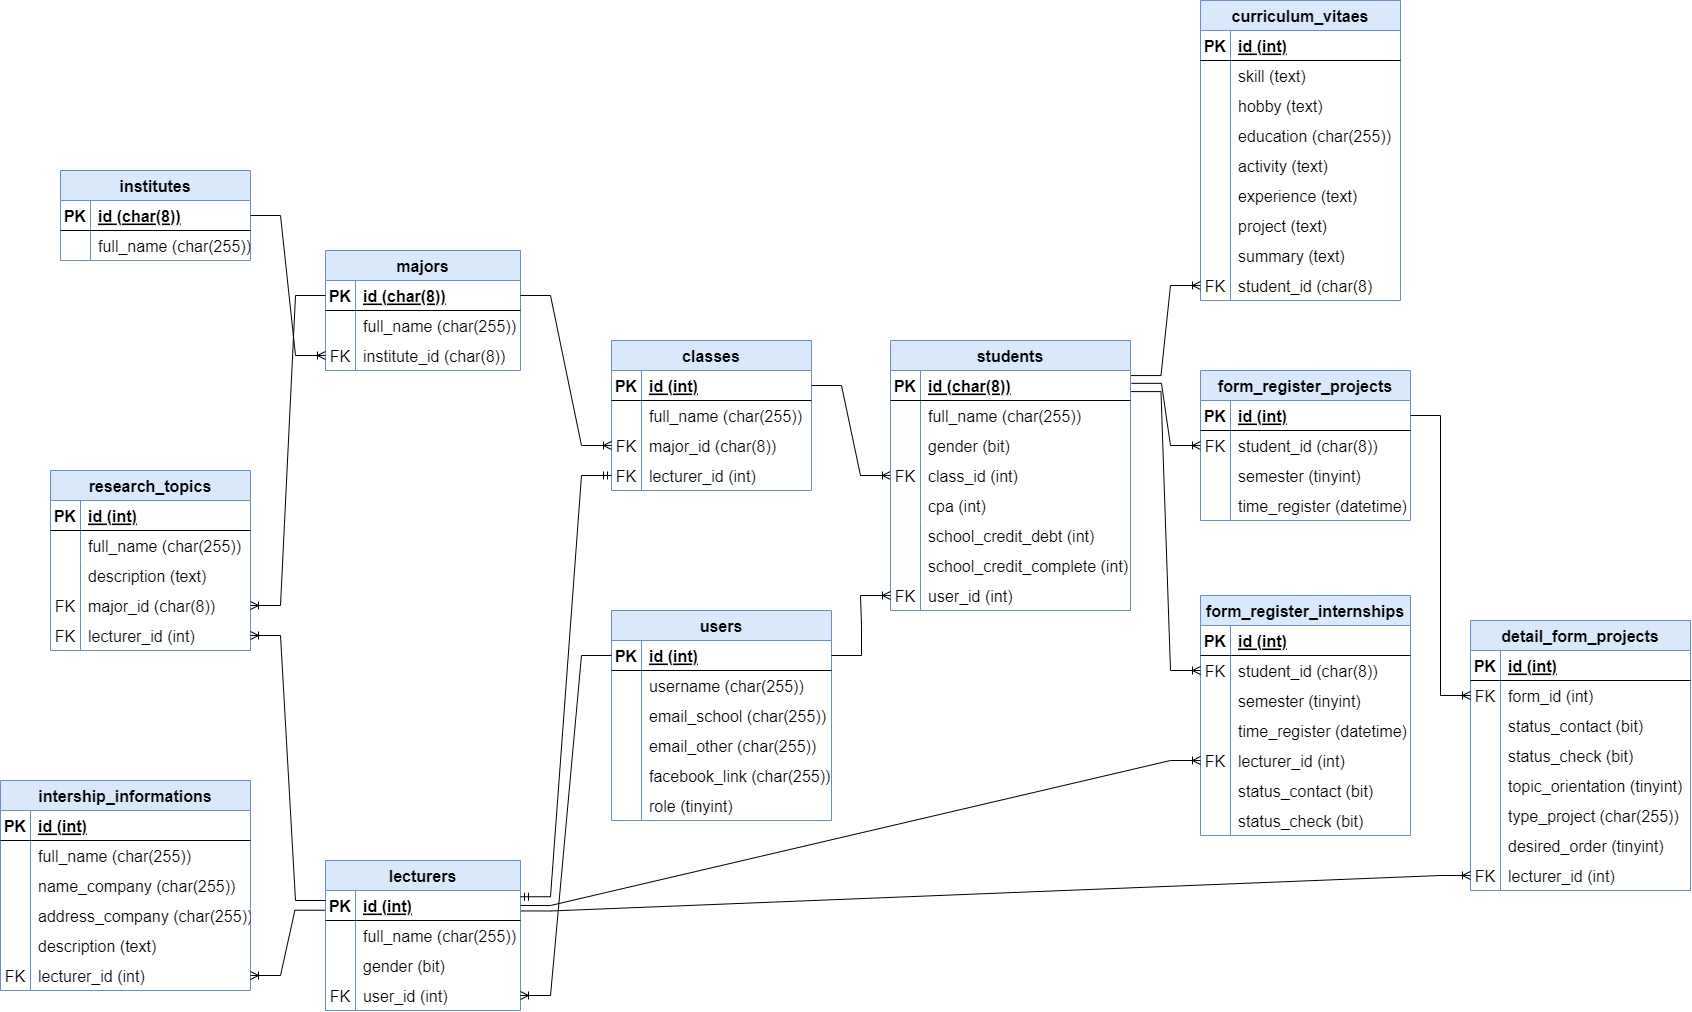
\includegraphics[width=1.5\textwidth]{../drawio/db_sv11.png}
    \begin{figure}[h]
      \centering
      \caption{Biểu đồ dữ liệu quan hệ}
    \end{figure}
  \end{center}
\end{landscape}

  \section{Giao diện}
    \subsection*{Một số giao diện quản trị viên}
    \begin{center}
      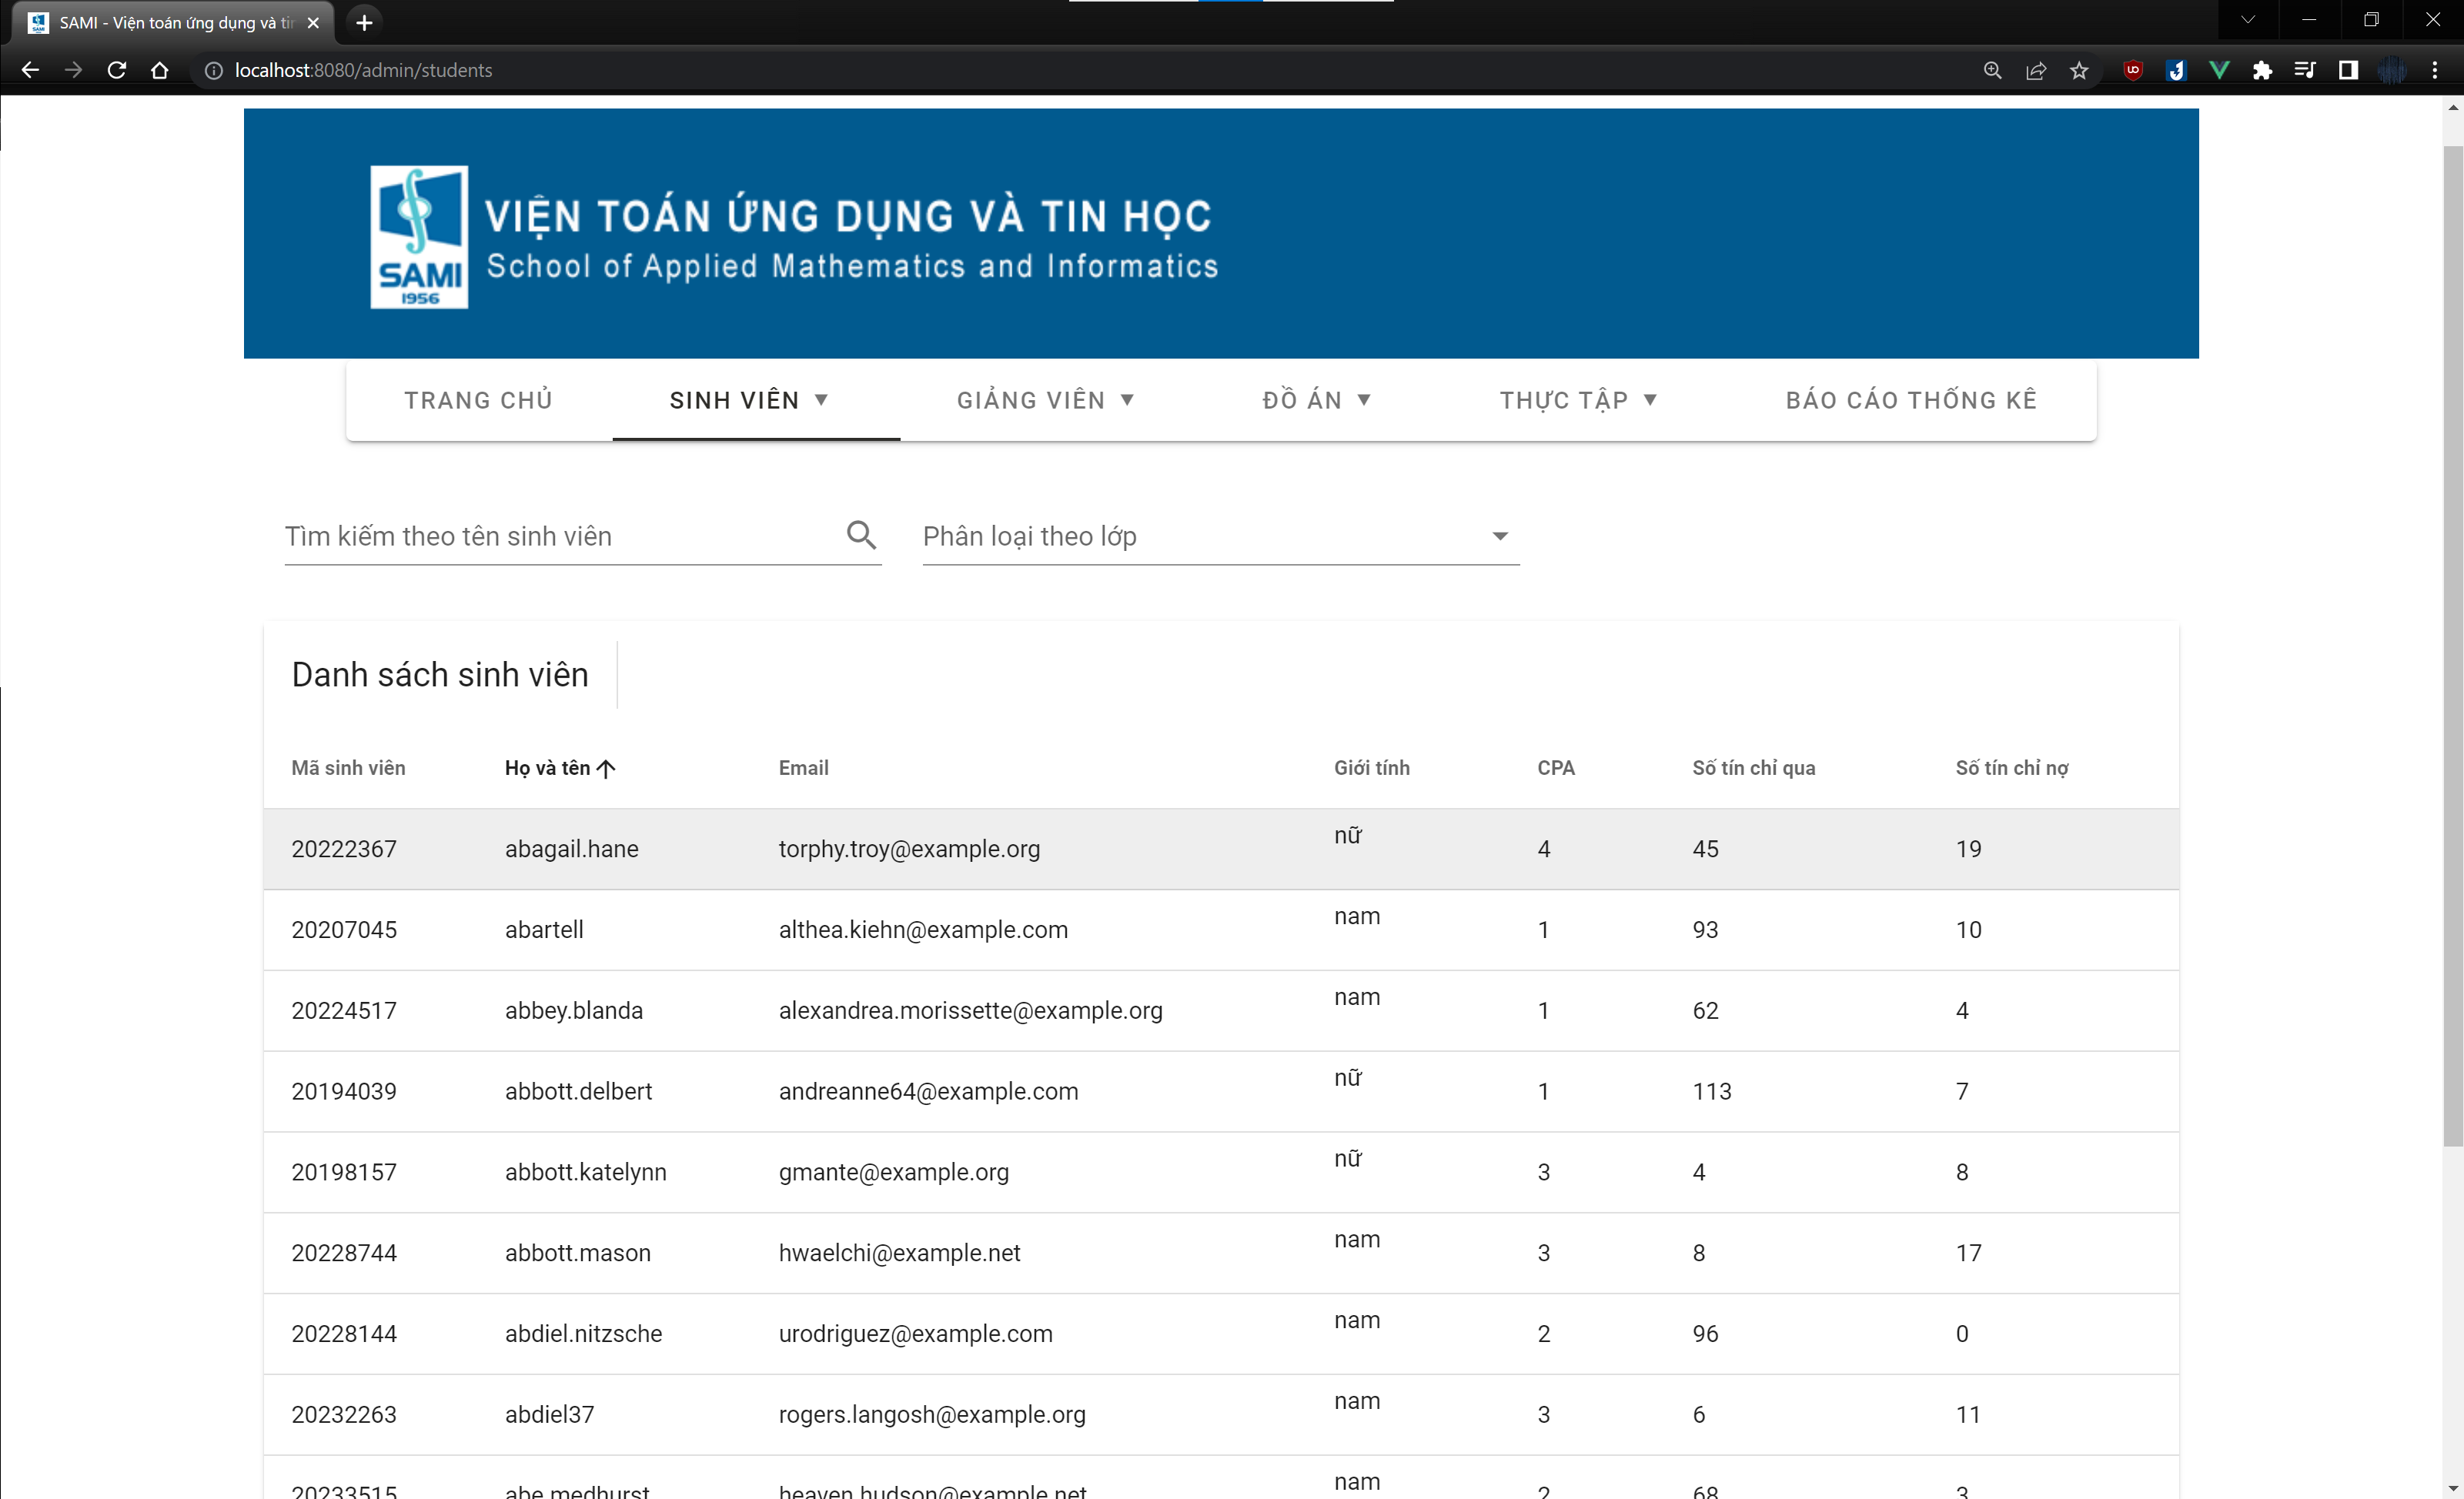
\includegraphics[width=.95\textwidth]{./image/design/admin/sv.png}
      \begin{figure}[h]
        \centering
        \caption{Giao diện quản lý sinh viên}
      \end{figure}
    \end{center}
    \begin{center}
      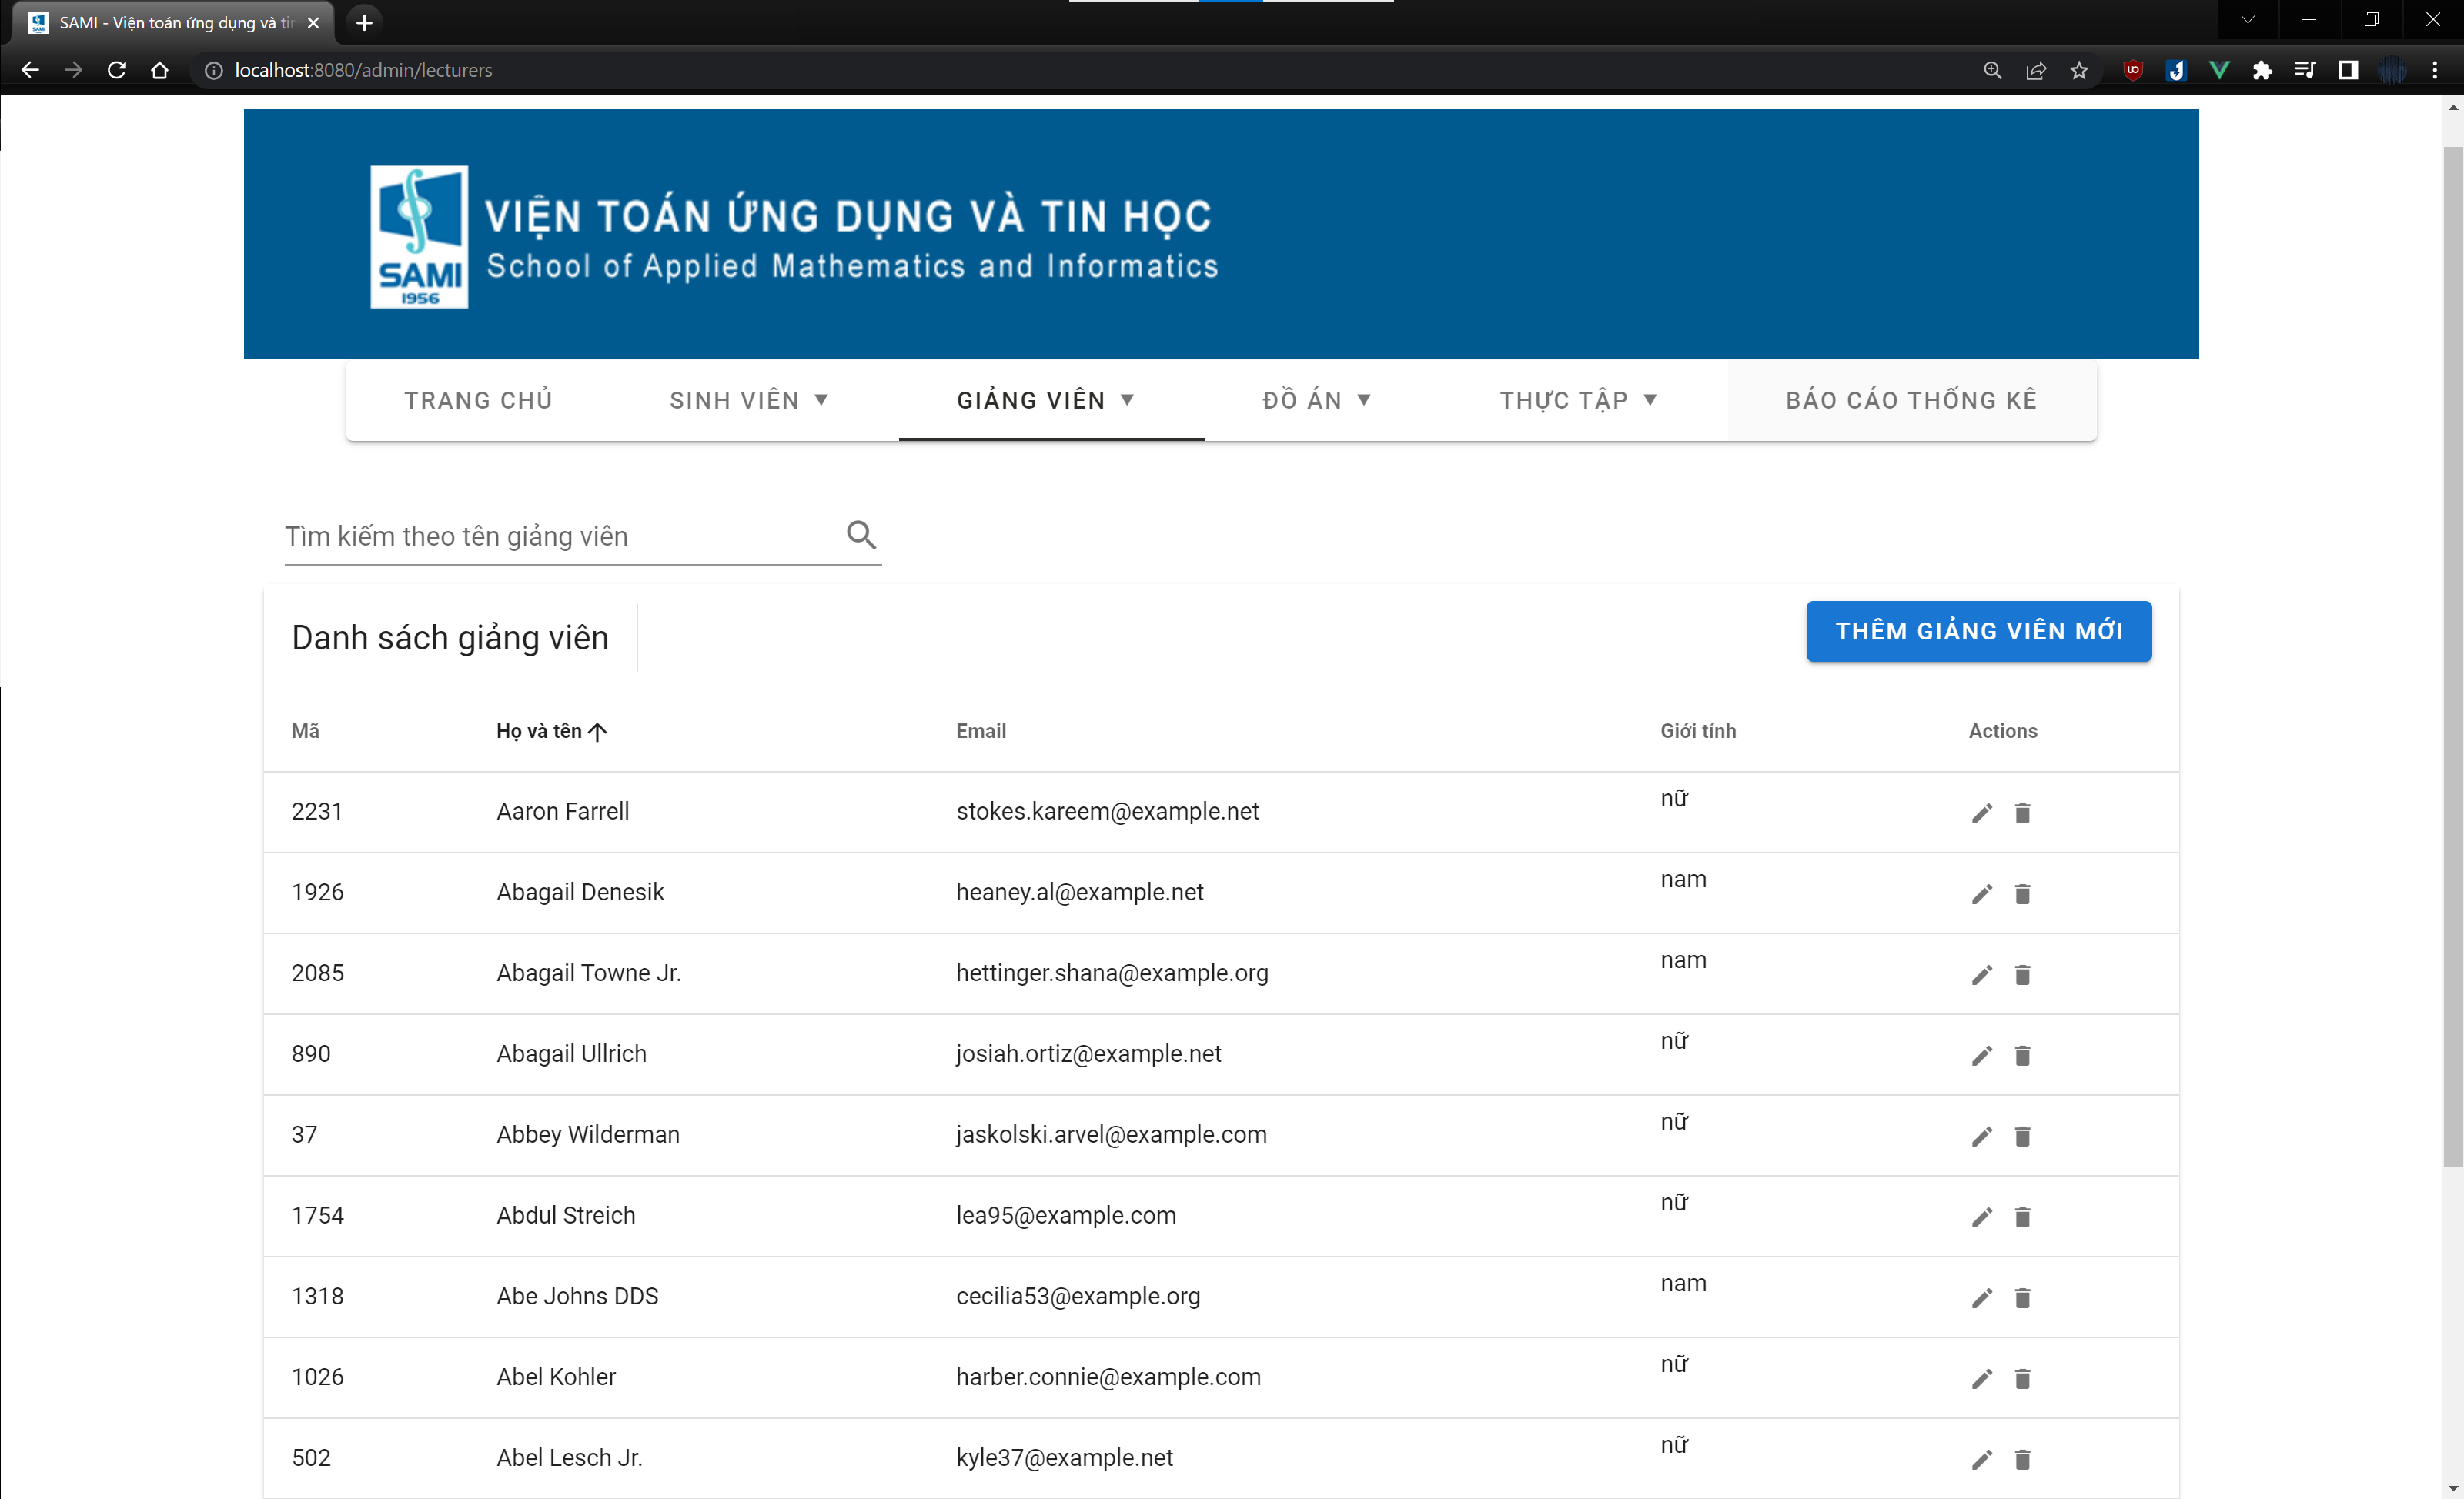
\includegraphics[width=.95\textwidth]{./image/design/admin/gv.png}
      \begin{figure}[h]
        \centering
        \caption{Giao diện quản lý giảng viên}
      \end{figure}
    \end{center}
    \begin{center}
      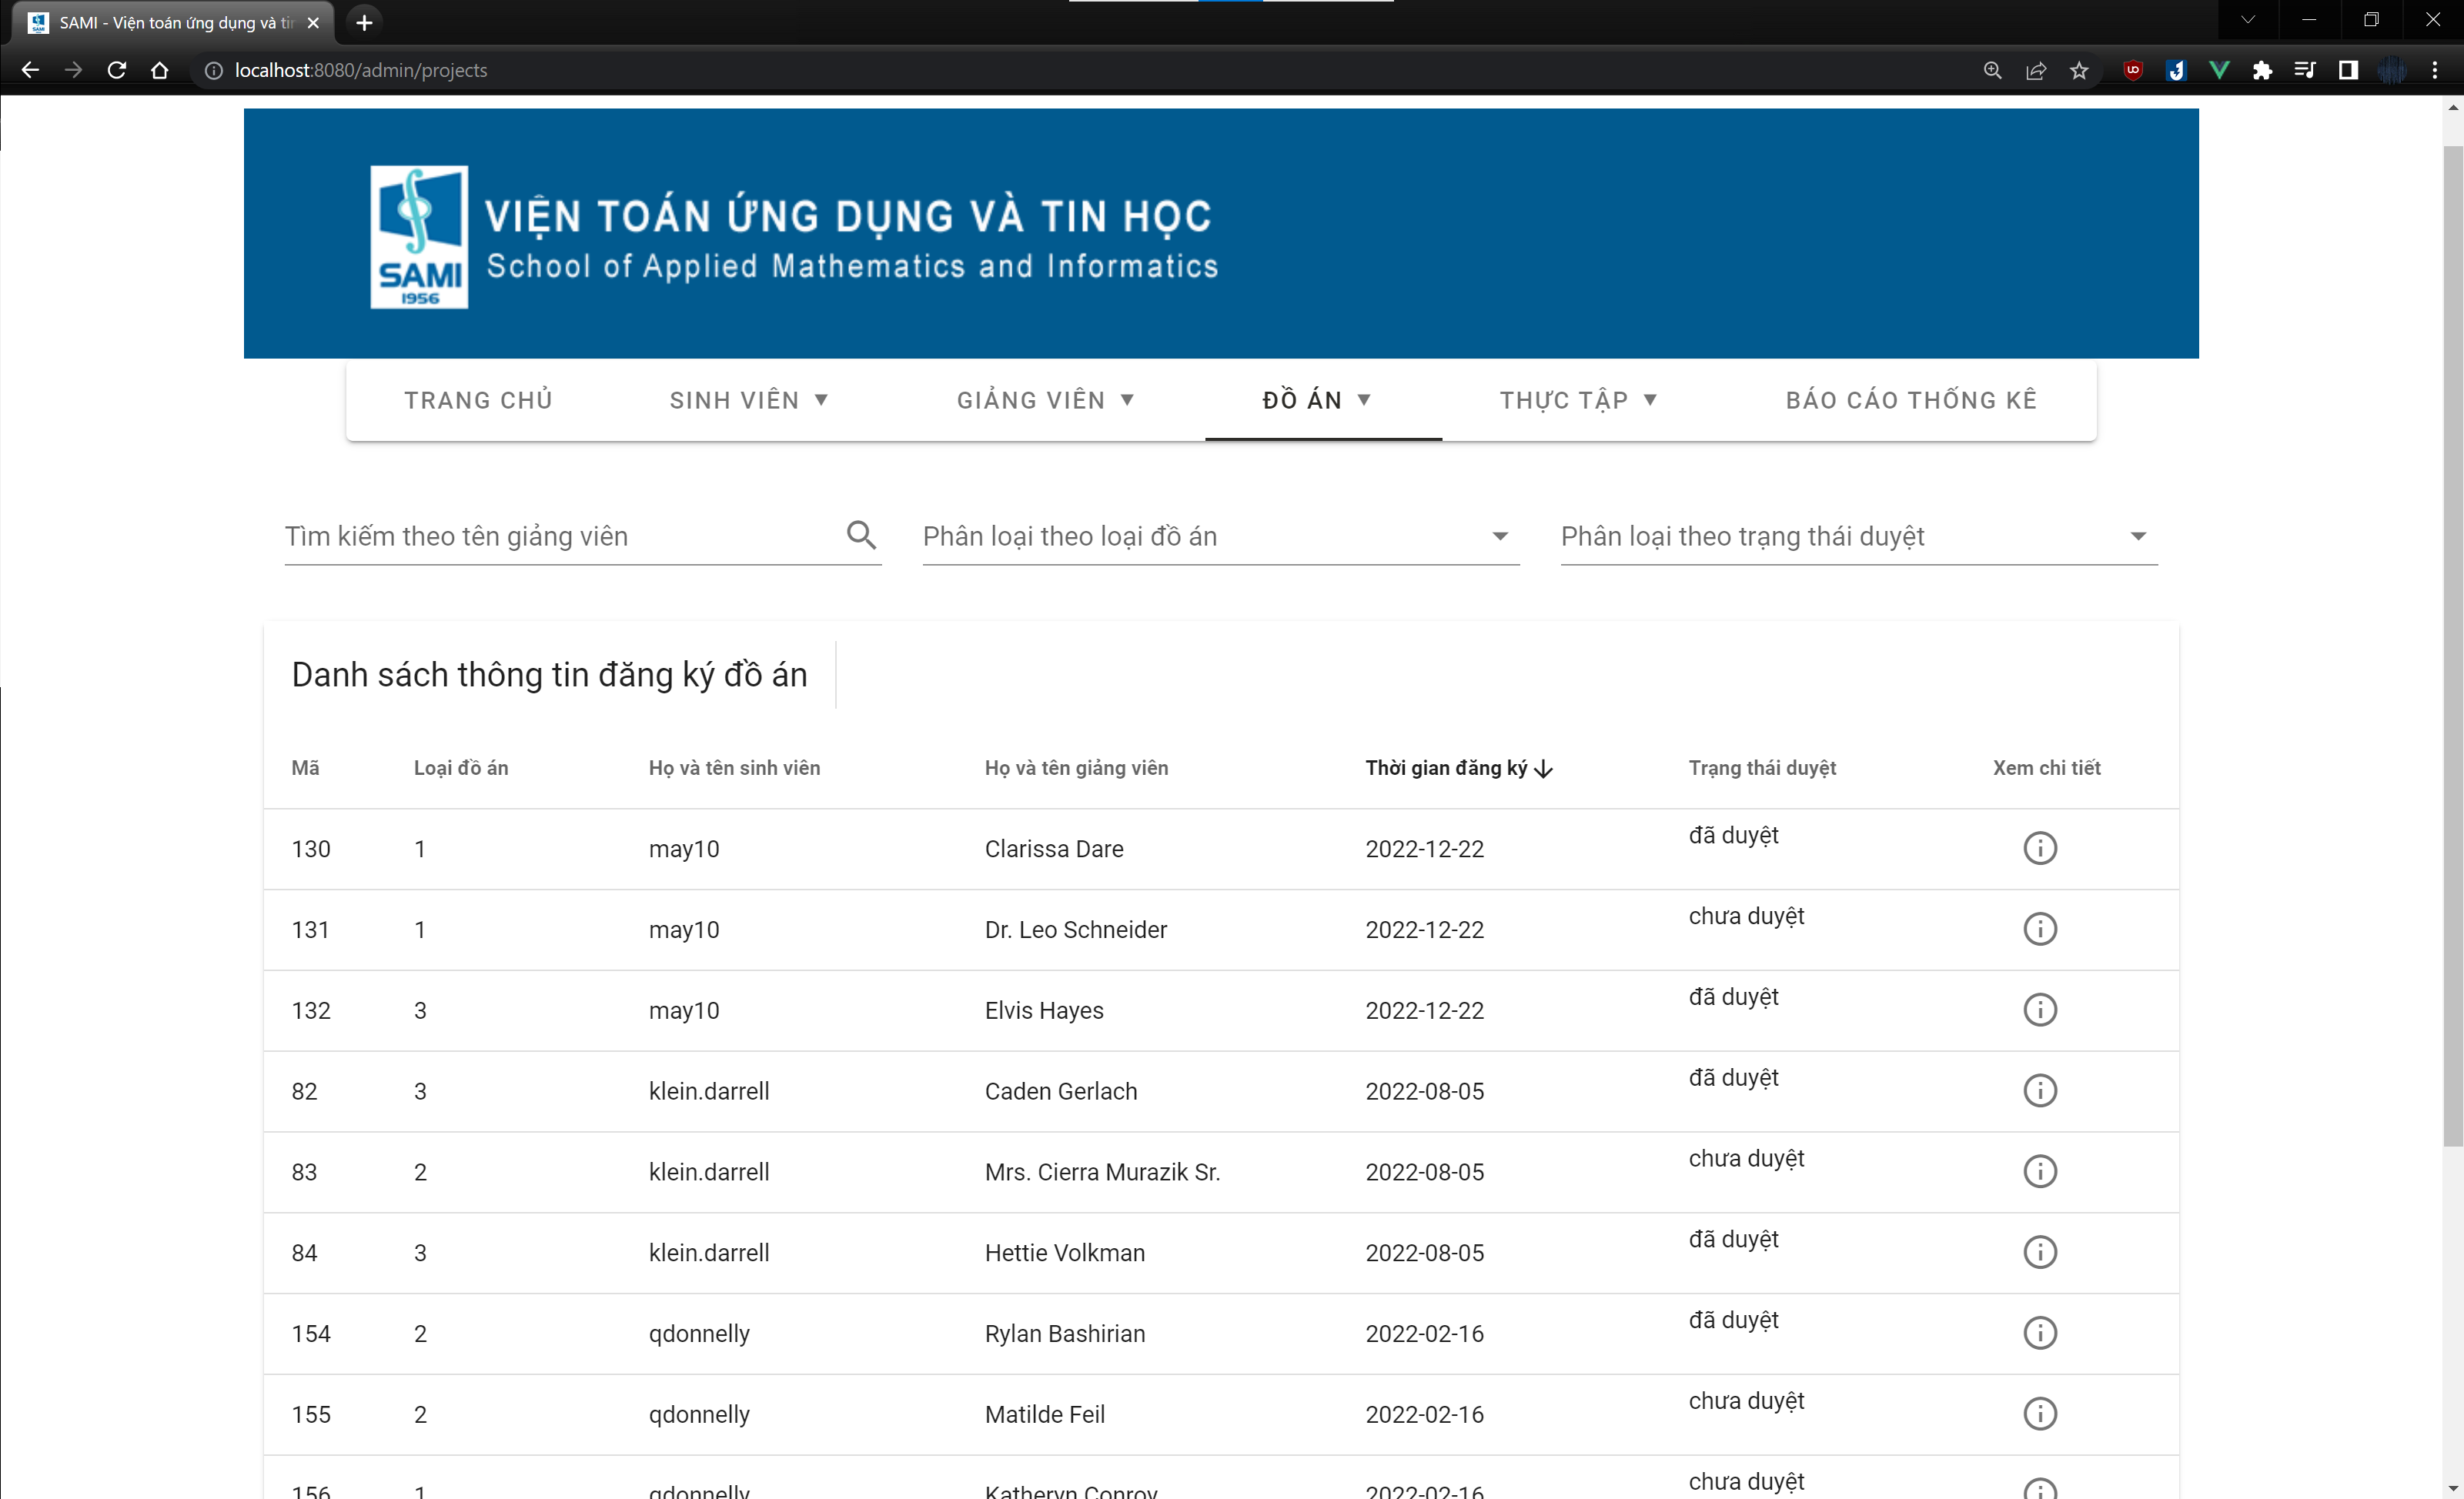
\includegraphics[width=1\textwidth]{./image/design/admin/da.png}
      \begin{figure}[h]
        \centering
        \caption{Giao diện quản lý thông tin đăng ký đồ án}
      \end{figure}
    \end{center}
    \begin{center}
      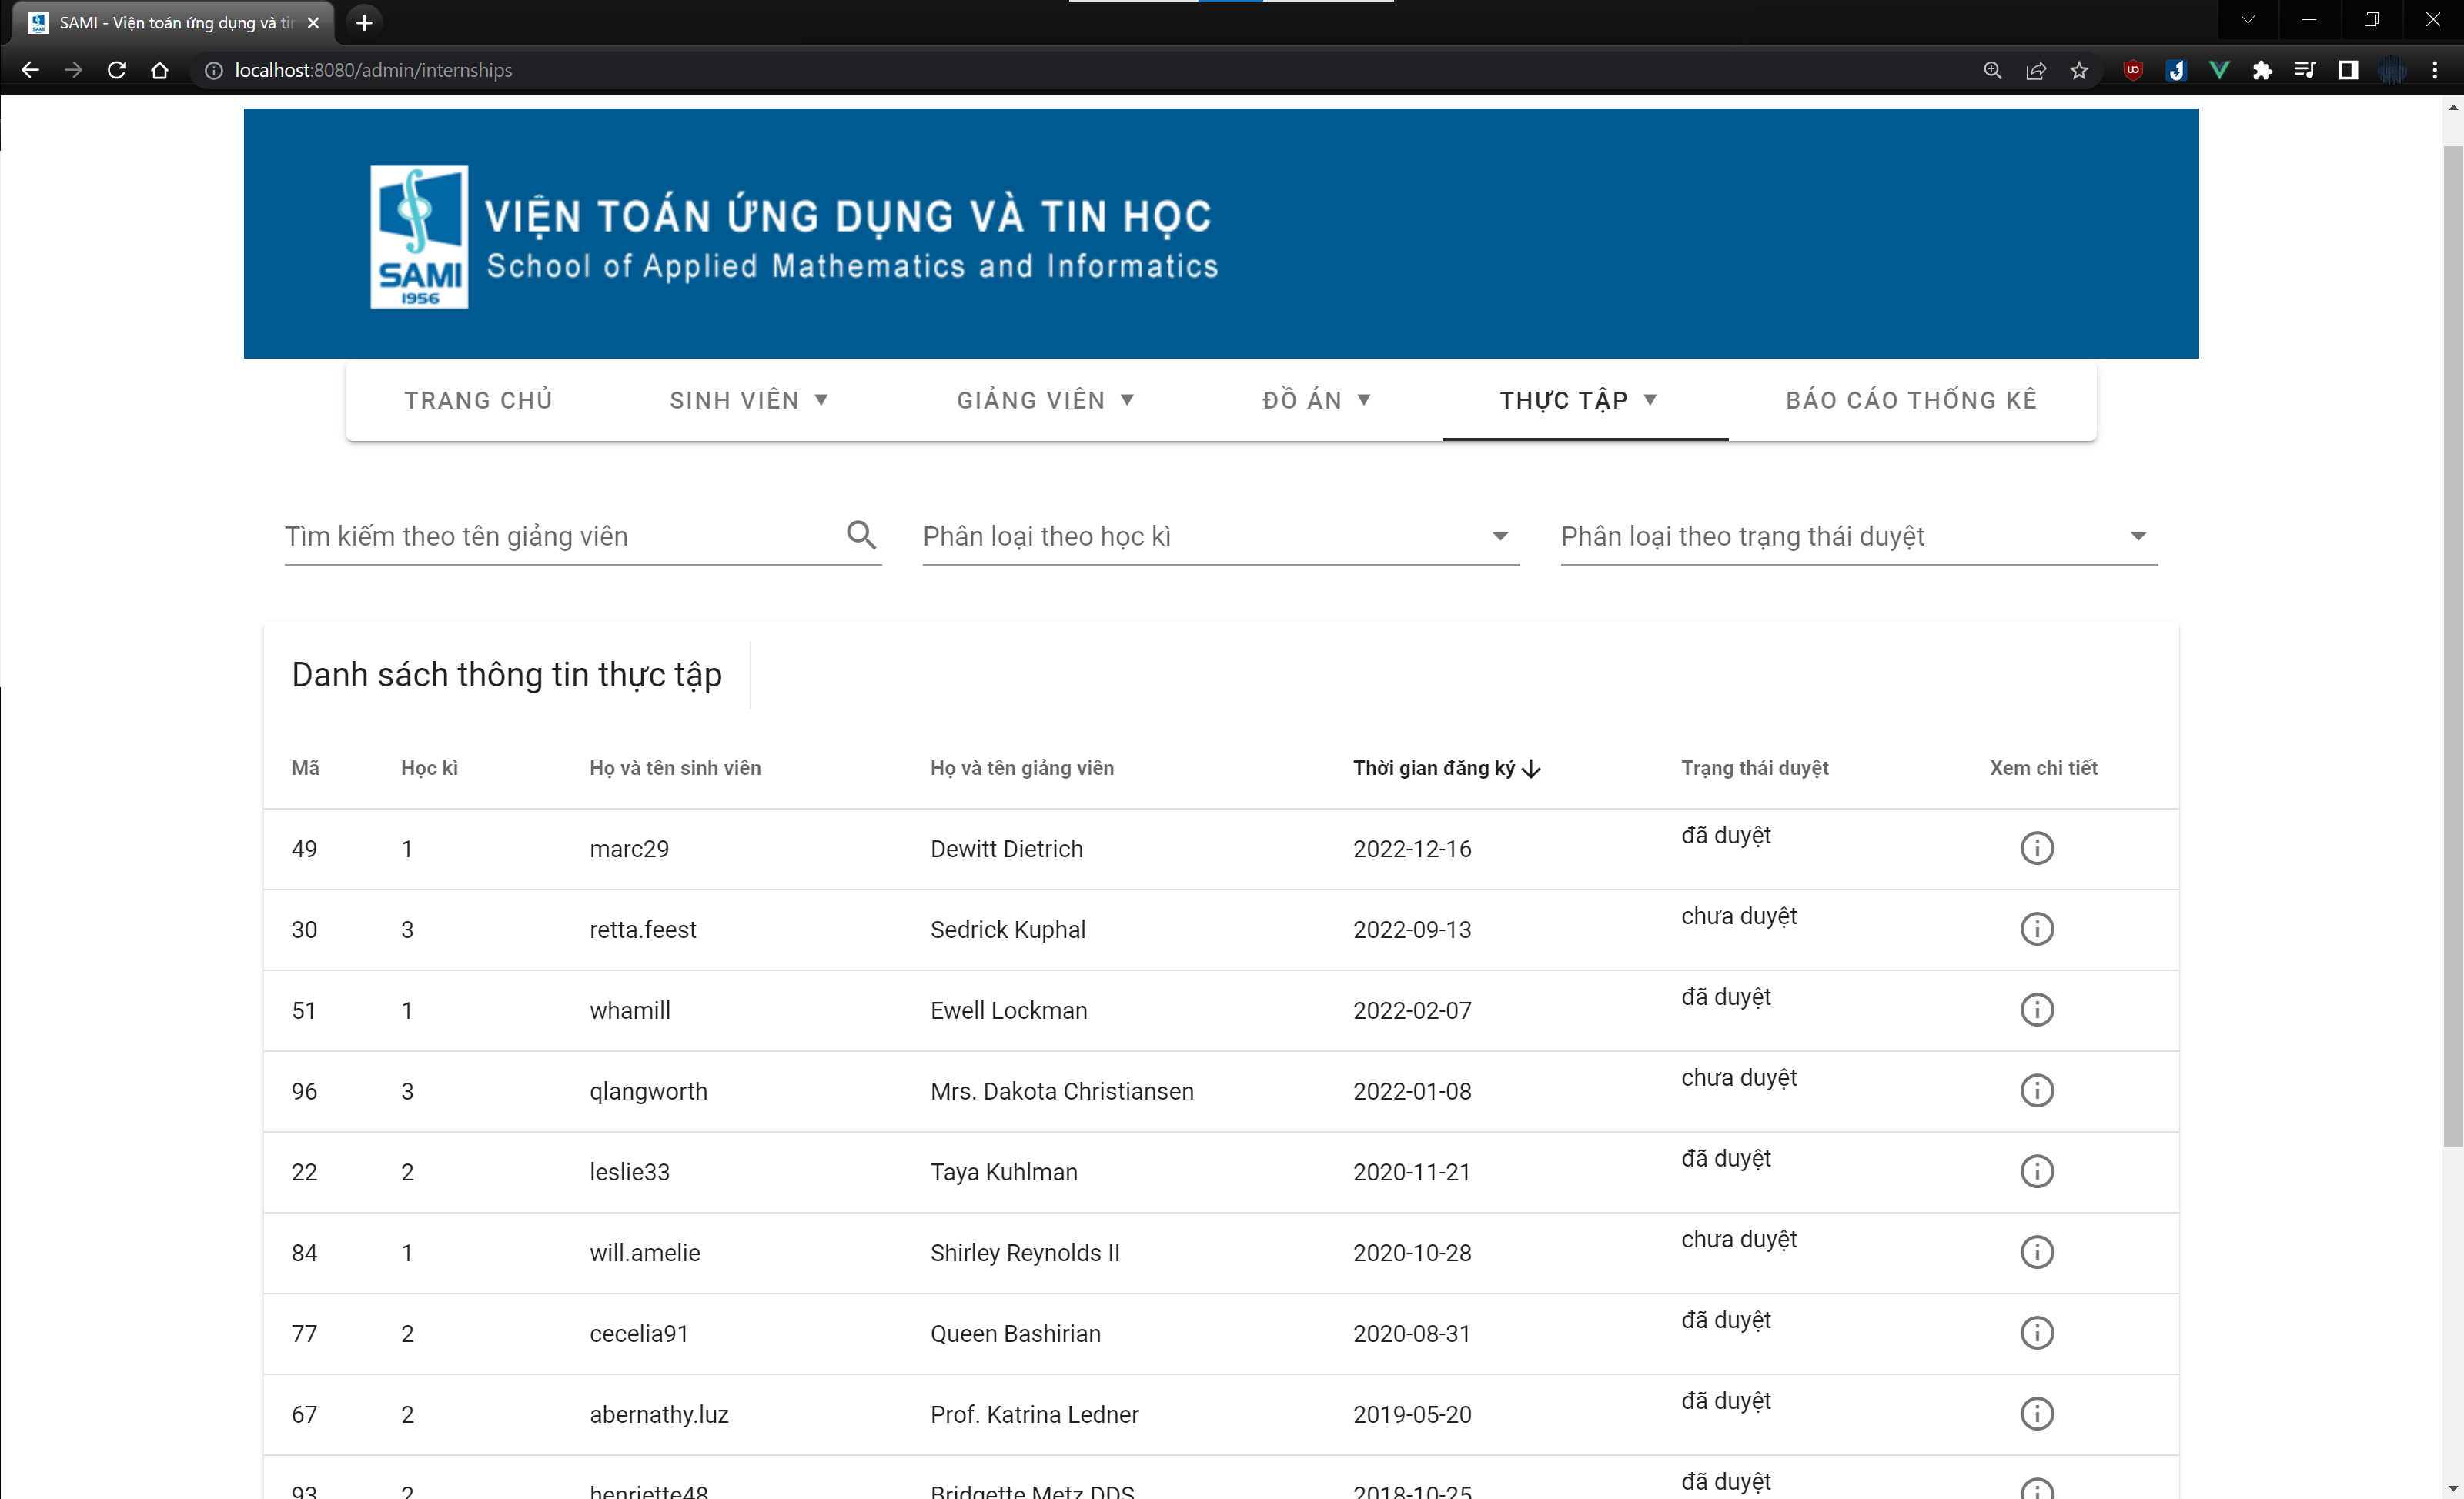
\includegraphics[width=1\textwidth]{./image/design/admin/tt.png}
      \begin{figure}[h]
        \centering
        \caption{Giao diện quản lý thông tin đăng ký thực tập}
      \end{figure}
    \end{center}
  \subsection*{Một số giao diện sinh viên}
    \begin{center}
      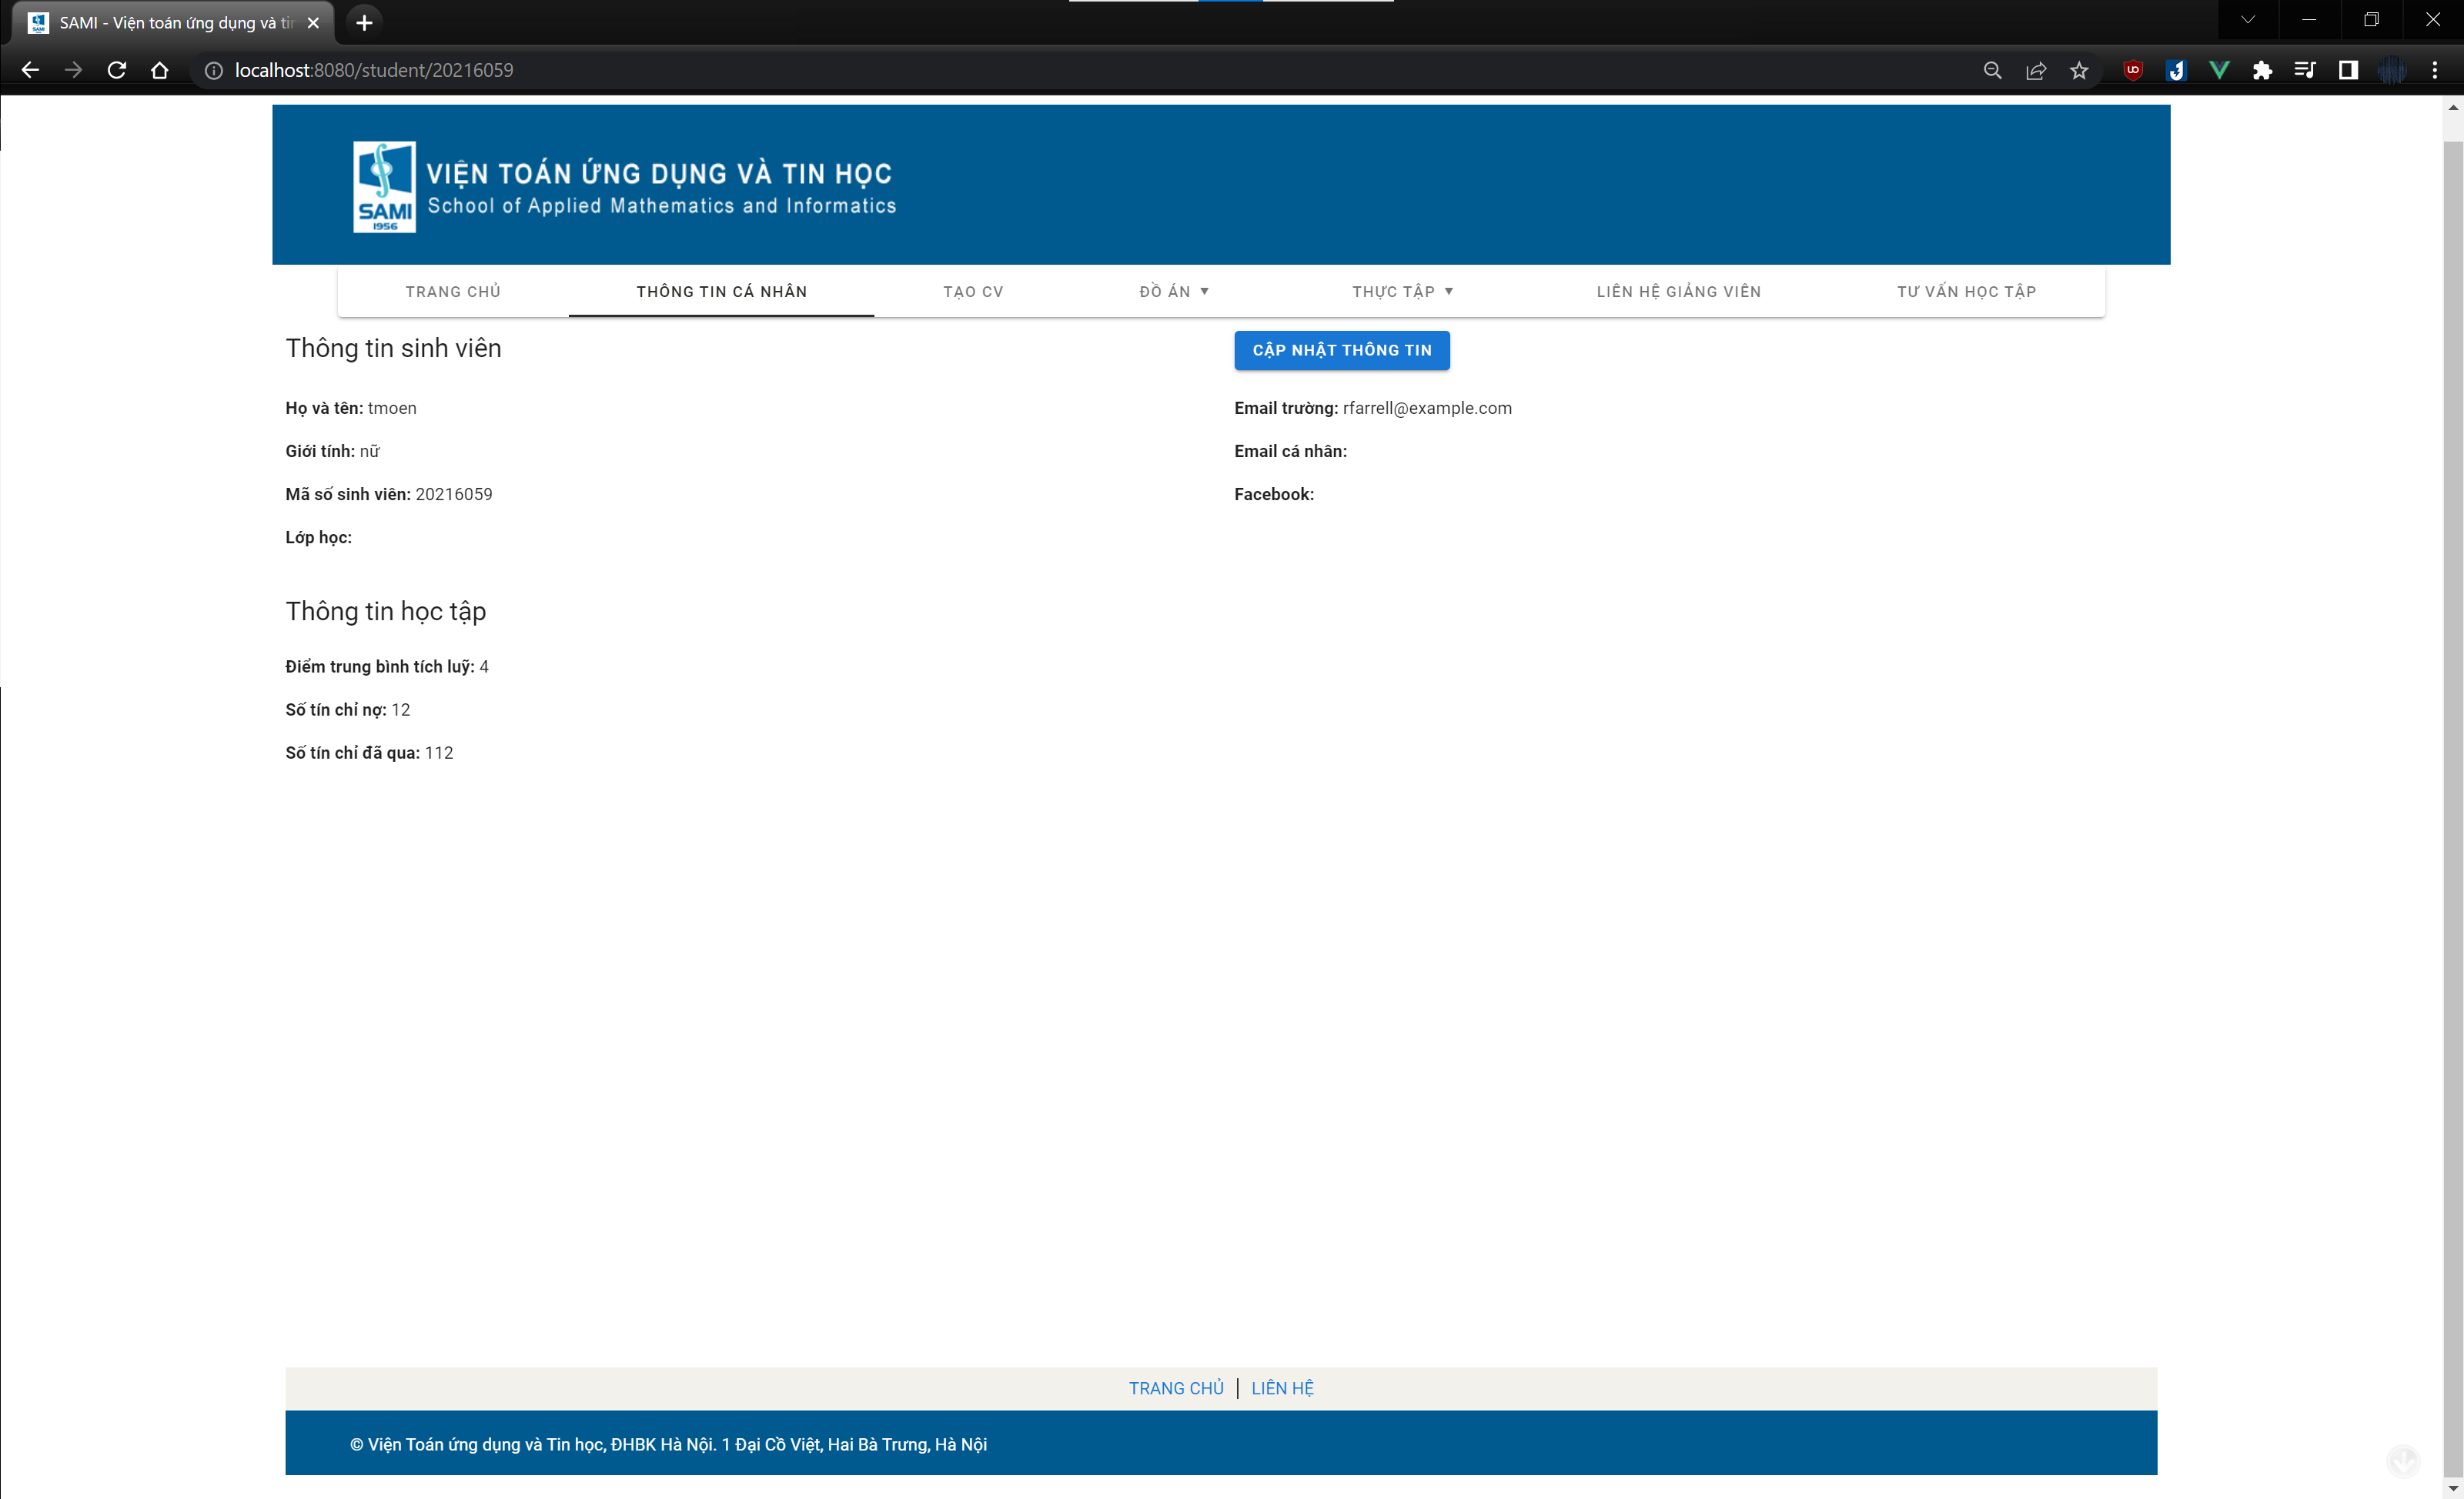
\includegraphics[width=.95\textwidth]{./image/design/student/info.png}
      \begin{figure}[h]
        \centering
        \caption{Giao diện thông tin sinh viên}
      \end{figure}
    \end{center}
    \begin{center}
      \includegraphics[width=1\textwidth]{./image/design/student/cv.png}
      \begin{figure}[h]
        \centering
        \caption{Giao diện điền thông tin tạo cv}
      \end{figure}
    \end{center}
    \begin{center}
      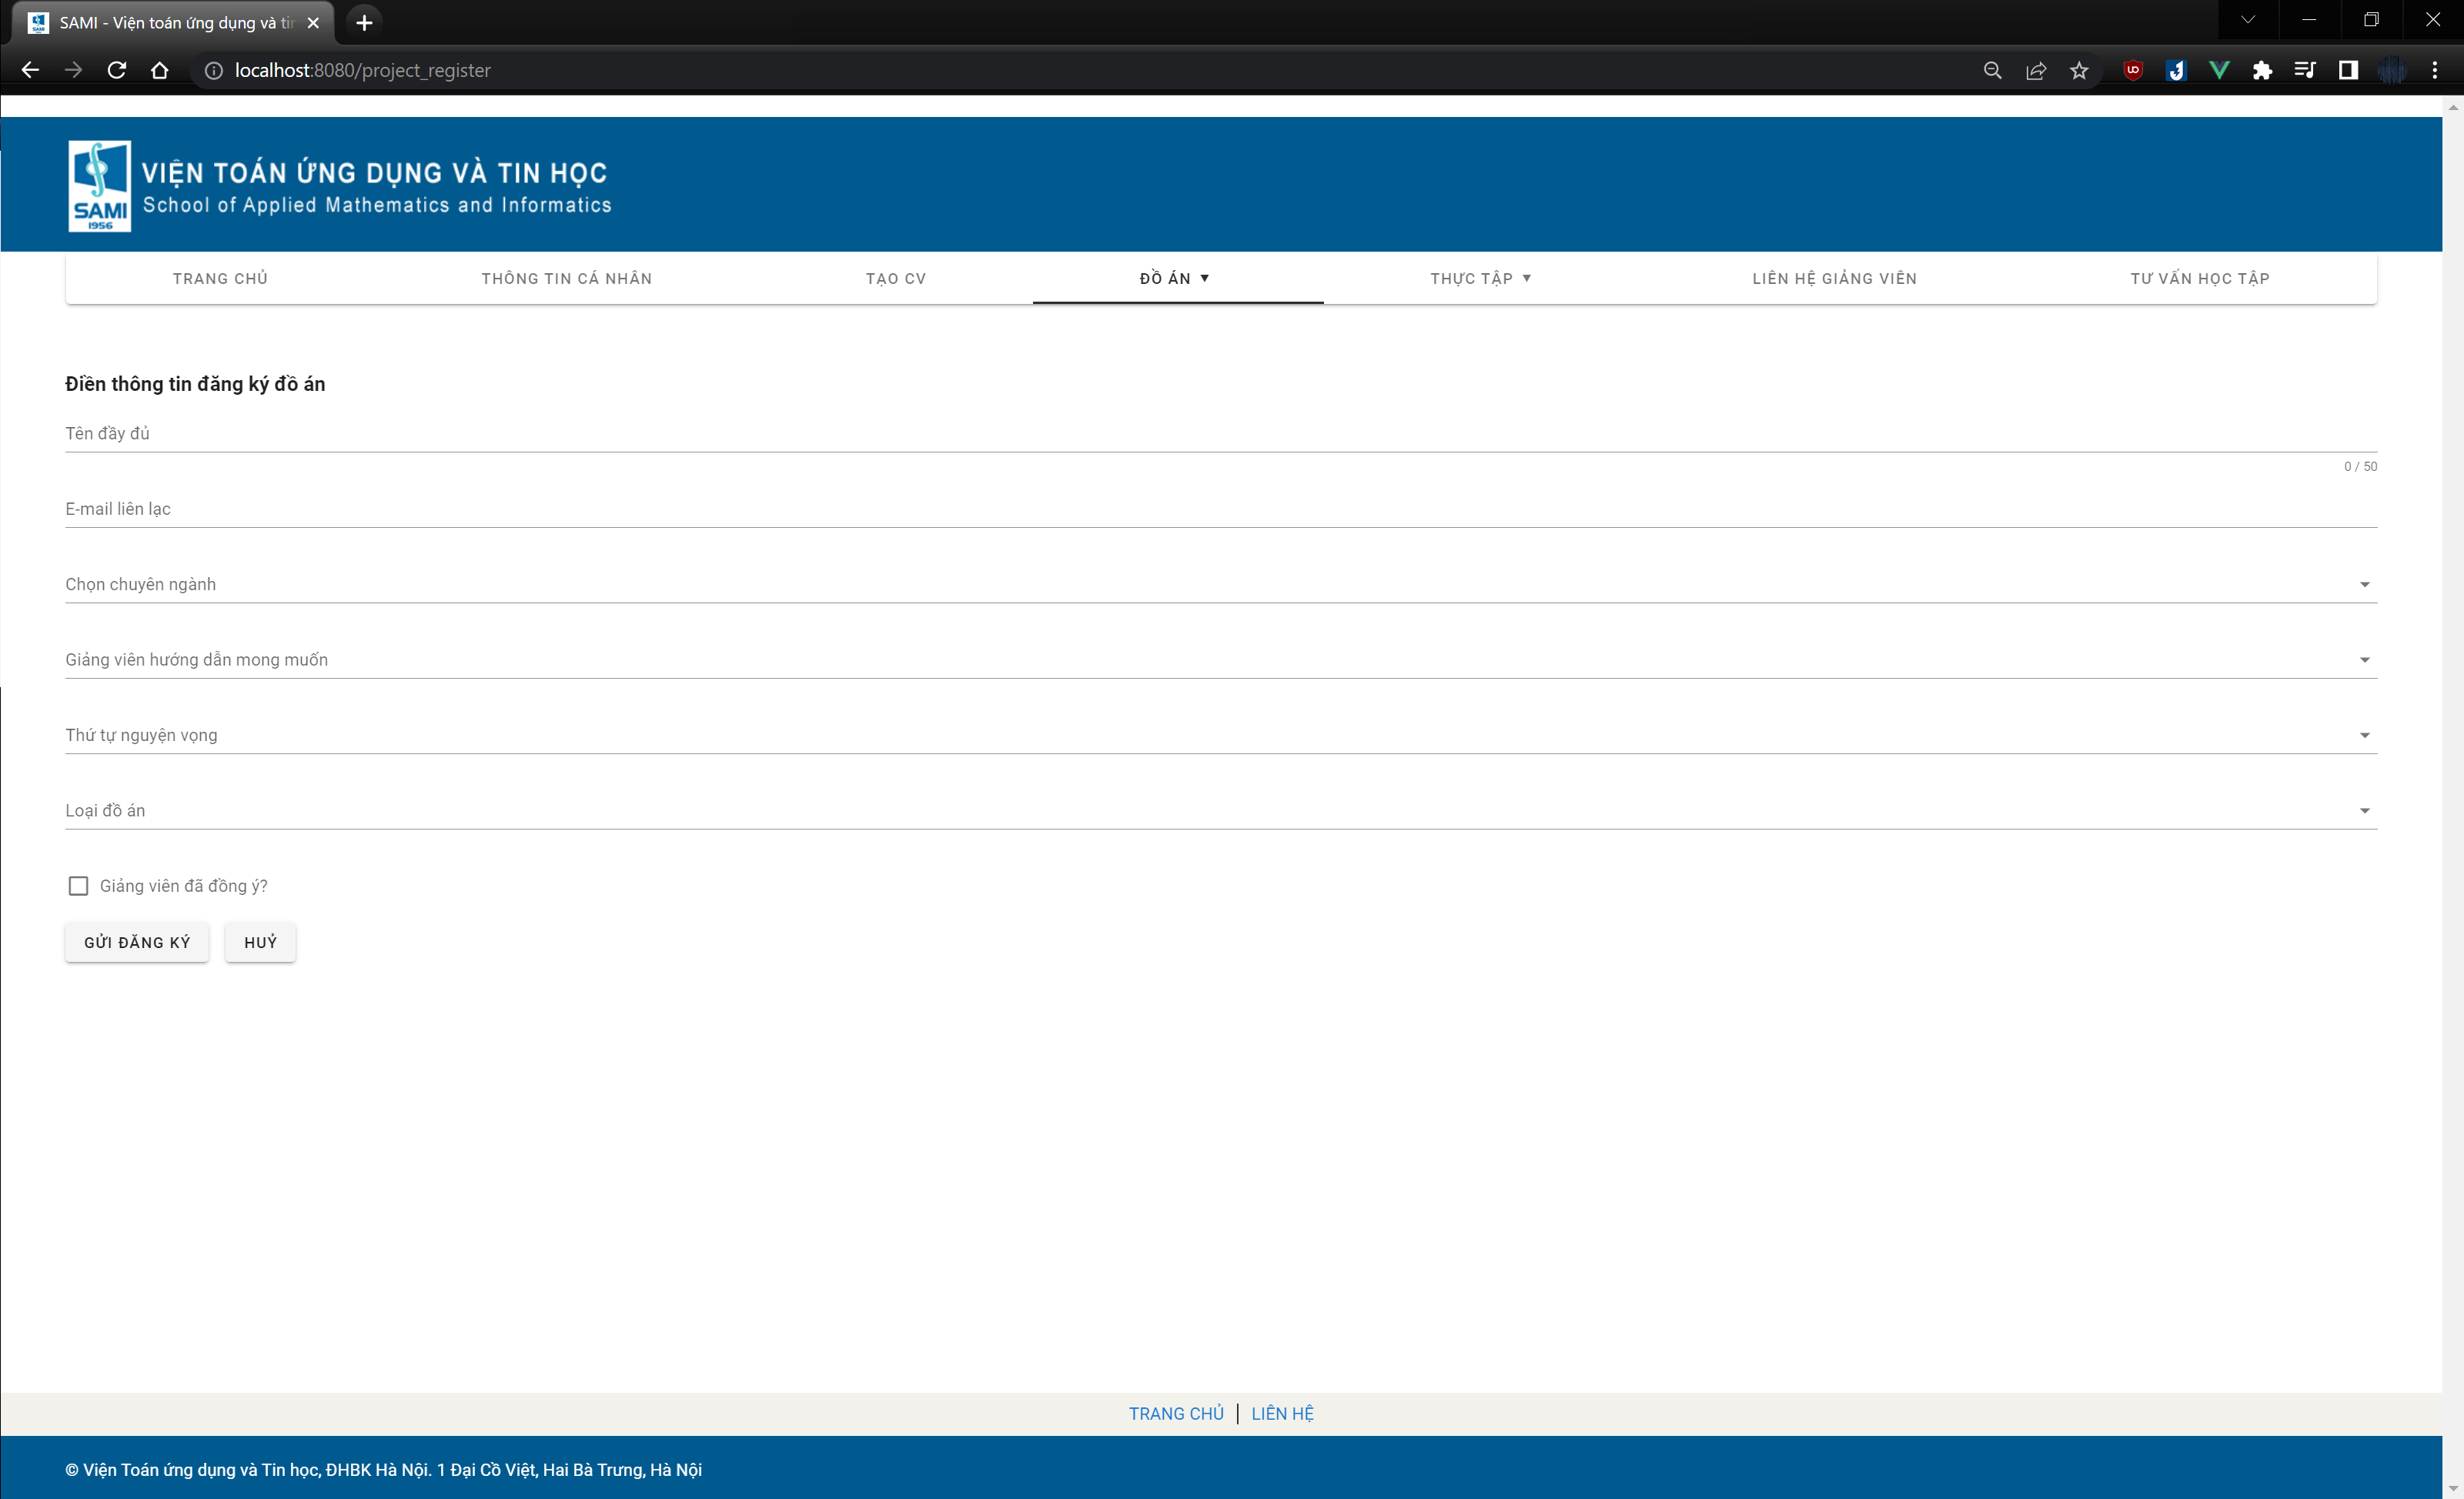
\includegraphics[width=1\textwidth]{./image/design/student/project.png}
      \begin{figure}[h]
        \centering
        \caption{Giao diện điền thông tin đăng ký đồ án}
      \end{figure}
    \end{center}
    % \subsection*{Một số giao diện giảng viên}
\chapter{Giao diện}
\chapter{Tổng kết}

\newpage

\begin{thebibliography}{9}
\thispagestyle{fancy}
\addcontentsline{toc}{chapter}{Tài liệu tham khảo}
    % \bibitem{MLcb} Machine Learning cơ bản - Vũ Hữu Tiệp
    \bibitem[label]{Quy chế đào tạo đại học hệ chính quy - Đại học Bách khoa Hà nội - Quyết định số 31/QĐ-ĐHBK-ĐTĐH ngày 21/3/2014}
    % \bibitem{taylor}Taylor: \textcolor{blue}{\url{https://www.le.ac.uk/users/dsgp1/COURSES/DERIVATE/TAYLOR.PDF}}
    \bibitem{taylor} Matt Kalinski, March 2022, "The Taylor Expansion", Theory and Applications of Trojan Wave Packets, Lab: Matt Kalinski's Lab.
    
\end{thebibliography}
%\cite{wiki}


\chapter{Đặc tả yêu cầu bài toán}
\section{Mô tả yêu cầu}
\subsection{Yêu cầu hệ thống quản lý sinh viên}
Xây dựng phần mềm quản lý thông tin sinh viên:
\begin{enumerate}
	\item Phầm mềm có yêu cầu đăng ký/đăng nhập hệ thống.
	\item Phầm mềm có thông tin lưu trữ của sinh viên: CPA, số tín chỉ đã qua, số tín chỉ nợ.
	\item Phần mềm có thể thống kê, đánh giá theo các mức cảnh báo sinh viên.
	\item Chức năng đăng ký hướng dẫn đồ án, thực tập.
	\item Chức năng tạo CV
	\item Chức năng tìm kiếm giảng viên, đề tài đồ án, vị trí thực tập.
\end{enumerate}

\subsection{Hệ thống quản lý sinh viên}
\begin{itemize}
	\item Chức năng đăng ký thành viên:
	      \begin{itemize}
		      \item Mỗi sinh viên đăng ký tài khoản mới với tài khoản microsoft mail trường cấp.
		      \item Đăng ký trực tiếp từ giao diện khởi động hệ thống.
		      \item Tài khoản đó sau khi đăng ký thành công có thể đăng nhập vào hệ thống.
		      \item Khi đăng ký thành công thì mặc định đó là tài khoản sinh viên.
	      \end{itemize}
	\item Chức năng đăng nhập/đăng xuất hệ thống có phân quyền người dùng:
	      \begin{itemize}
		      \item Tài khoản đăng nhập hệ thống với đúng tài khoản và mật khẩu mà hệ thống cung cấp.
		      \item Có thể đăng nhập bằng tài khoản google gmail hoặc tài khoản facebook trước đó đã được liên kết với tài khoản đăng ký.
		      \item Tài khoản đăng nhập nếu không còn nhu cầu sử dụng hệ thống hoặc cần đăng nhập tài khoản khác có thể tiến hành đăng xuất.
	      \end{itemize}
	\item Chức năng lưu trữ thông tin:
	      \begin{itemize}
		      \item Sinh viên có thể cập nhật, lưu trữ các thông tin học tập của cá nhân: CPA, số tín chỉ đã qua, số tín chỉ nợ, thuộc lớp nào.
		      \item Cán bộ giảng viên phụ trách có thể xem danh sách lớp và xác nhận sinh viên.
	      \end{itemize}
	\item Chức năng cập nhật thông tin:
	      \begin{itemize}
		      \item Hệ thống cho phép người dùng thay đổi thông tin cá nhân của mình.
		      \item Admin có thể cấp lại mật khẩu cho người dùng.
	      \end{itemize}
	\item Chức năng thống kê, đưa ra mức cảnh báo:
	      \begin{itemize}
		      \item Hệ thống có thể đưa ra biểu đồ thống kê số lượng các sinh viên đang ở các mức cảnh báo 1, 2, 3 và các sinh viên chậm chương trình.
		      \item Hệ thống có thể xuất dữ liệu ra file excel, pdf.
	      \end{itemize}
	\item Chức năng đăng ký hướng dẫn đồ án, thực tập:
	      \begin{itemize}
		      \item Hệ thống cung cấp form đăng ký hướng dẫn đồ án, form đăng ký thực tập.
		      \item Giáo vụ có thể kiểm tra các form đã submit về.
		      \item Trưởng bộ môn có thể truy cấp để xếp thứ tự ưu tiên các sinh viên.
	      \end{itemize}
	\item Chức năng tạo CV:
	      \begin{itemize}
		      \item Hệ thống cung cấp form để sinh viên điền các thông tin cá nhân của mình: giới thiệu bản thân, CPA, định hướng nghề nghiệp, kỹ năng hiện có,...
		      \item Hệ thống nhận form submit và trả về một file word bản CV mẫu, sinh viên có thể tải xuống để xem, chỉnh sửa.
	      \end{itemize}
	\item Chức năng tìm kiếm giảng viên, đề tài đồ án, vị trí thực tập:
	      \begin{itemize}
		      \item Hệ thống cho phép tìm kiếm từ khoá theo tên giảng viên, từ đó đưa ra các đề tài mà giảng viên hướng dẫn
		      \item Hệ thống cung cấp danh sách các vị trí thực tập.
	      \end{itemize}
\end{itemize}


\chapter{Phân tích các biểu đồ}
\section{Biểu đồ phân cấp chức năng}
\begin{center}
	\includegraphics[width=1.1\textwidth]{image/BDPCCN.png}
	\begin{figure}
		\centering
		\caption{biểu đồ phân cấp chức năng}
	\end{figure}
\end{center}

\section{Biểu đồ usecase}
\begin{center}
	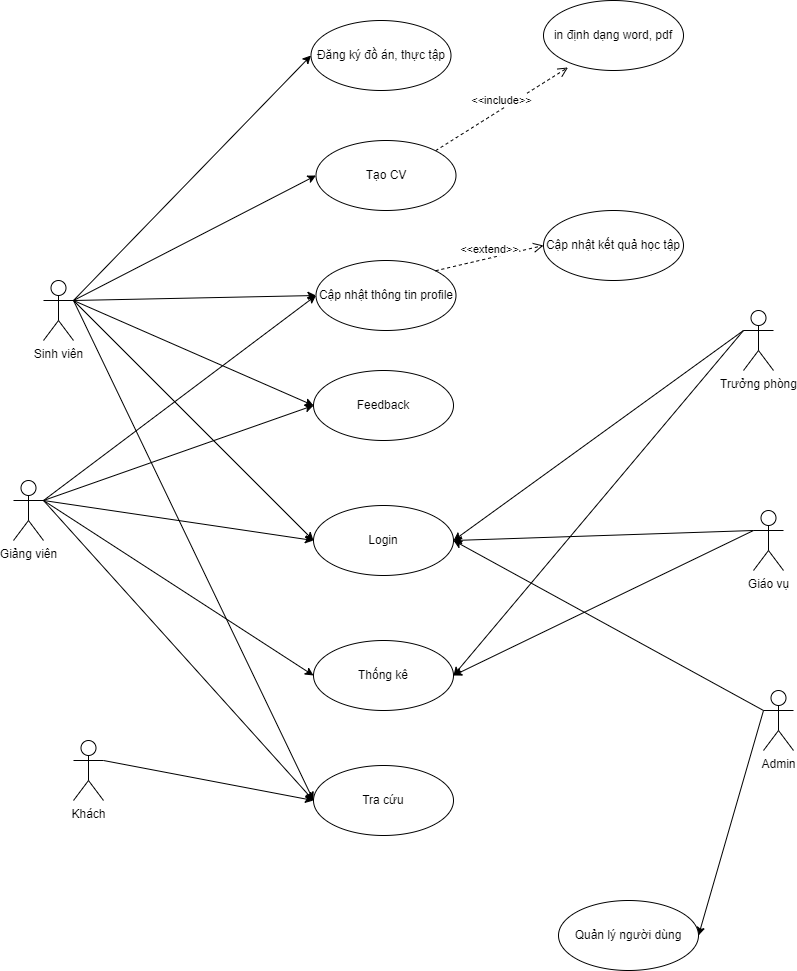
\includegraphics[width=1.\textwidth]{../drawio/usecase.png}
	\begin{figure}[h]
		\centering
		\caption{biểu đồ usecase}
	\end{figure}
\end{center}

\section{Biểu đồ lớp}
\begin{center}
	\includegraphics[width=1.2\textwidth]{../out/plantUML/class/class.png}
	\begin{figure}[h]
		\centering
		\caption{biểu đồ lớp}
	\end{figure}
\end{center}

\section{Đặc tả usecase}
	\subsection*{Đăng nhập}
		\begin{tabular}{|l|p{0.7\textwidth}|}
			\hline
			\textbf{Các tác nhân}         & Admin, sinh viên, giảng viên, cán bộ \\
			\hline
			\textbf{Mô tả}                & Đăng nhập                                           \\
			\hline
			\textbf{Kích hoạt}            & Người dùng nhấn vào nút "Đăng nhập" trên thanh menu \\
			\hline
			\textbf{Luồng chính}          & \makecell[l]{1. Chọn chức năng đăng nhập            \\ 2. Hiển thị màn hình đăng nhập \\ 3. Nhập tên đăng nhập và mật khẩu \\ 4. Hiển thị kiểm tra thông tin \\ 5. Nếu thành công chuyển tới giao diện chính \\ 6. Kết thúc} \\
			\hline
			\textbf{Các luồng thay thế}   & \makecell[l]{Mật khẩu không hợp lệ:                 \\ 1. Thông báo ra màn hình mật khẩu sai \\ 2. Quay lại bước 2 của luồng chính \\ Quên mật khẩu: \\ 1. Hiển thị màn hình nhập email \\ 2. Nhập và chọn chức năng quên mật khẩu \\ 3. Kiểm tra hợp lệ hệ thống gửi mail xác nhận \\ 4. Hiển thị thông báo thành công \\ 5. Kết thúc} \\
			\hline
			\textbf{Tiền điều kiện}       & Tài khoản trước đó đã được đăng ký                  \\
			\hline
			\textbf{Hậu điều kiện}        & Người dùng đăng nhập thành công                     \\
			\hline
			\textbf{Các yêu cầu đặc biệt} &                                                     \\
			\hline
		\end{tabular}

	\subsection*{Đăng ký}
	\begin{tabular}{|l|p{0.7\textwidth}|}
		\hline
		\textbf{Các tác nhân}       & Admin, sinh viên, giảng viên                                        \\
		\hline
		\textbf{Mô tả}              & Đăng ký                                                             \\
		\hline
		\textbf{Kích hoạt}          & Người dùng nhấn vào nút "Đăng ký" trên thanh menu                   \\
		\hline
		\textbf{Luồn chính}         & \makecell[l]{Trường hợp bắt đầu khi người truy cập muốn đăng ký tài \\khoản mới: \\ 1. Chọn chức năng đăng ký \\ 2. Màn hình hiển thị form đăng ký \\ 3. Hệ thống nhận các thông tin, thực hiện validate \\ 4. Thông báo đăng ký thành công \\ 5. Kết thúc} \\
		\hline
		\textbf{Các luồng thay thế} & \makecell[l]{Đăng ký thất bại:                                      \\ - Thông tin đăng ký không hợp lệ \\ - Email đã được đăng ký} \\
		\hline
		\textbf{Tiền điều kiện}     & Người dùng trước đó đã đăng nhập                                    \\
		\hline
		\textbf{Hậu điều kiện}      & Người dùng đăng xuất thành công                                     \\
		\hline
		\textbf{Yêu cầu đặc biệt}   &                                                                     \\
		\hline
	\end{tabular}

	\subsection*{Đăng xuất}
	\begin{tabular}{|l|p{0.7\textwidth}|}
		\hline
		\textbf{Các tác nhân}         & Admin, sinh viên, giảng viên, cán bộ                              \\
		\hline
		\textbf{Mô tả}                & Đăng xuất                                                                        \\
		\hline
		\textbf{Kích hoạt}            & Người dùng nhấn vào nút "Đăng xuất" trên thanh menu                              \\
		\hline
		\textbf{Luồn chính}           & \makecell[l]{Trường hợp bắt đầu khi người truy cập muốn đăng xuất \\ khỏi hệ thống: \\ 1. Chọn chức năng đăng xuất \\ 2. Màn hình hiển thị thông báo xác nhận muốn đăng xuất \\ 3. Thông báo đăng xuất thành công \\ 4. Kết thúc} \\
		\hline
		\textbf{Các luồng thay thế}   & Không có                                                                         \\
		\hline
		\textbf{Tiền điều kiện}       & Người dùng trước đó đã đăng nhập                                                 \\
		\hline
		\textbf{Hậu điều kiện}        & Người dùng đăng xuất thành công                                                  \\
		\hline
		\textbf{Các yêu cầu đặc biệt} &                                                                                  \\
		\hline
	\end{tabular}

	\subsection*{Quên mật khẩu}
	\begin{tabular}{|l|p{0.7\textwidth}|}
		\hline
		\textbf{Các tác nhân}         & Sinh viên, giảng viên, cán bộ                            \\
		\hline
		\textbf{Mô tả}                & Quên mật khẩu                                           \\
		\hline
		\textbf{Kích hoạt}            & Người dùng nhấn vào nút "Quên mật khẩu" trên thanh menu \\
		\hline
		\textbf{Luồn chính}           & \makecell[l]{1. Người dùng chọn chức năng quên mật khẩu \\ 2. Hệ thống tiếp nhận thông tin email \\ 3. Hệ thống kiểm tra email \\ 4. Hệ thống thông báo mật khẩu mới được gửi qua email \\ 5. Kết thúc} \\
		\hline
		\textbf{Các luồng thay thế}   & \makecell[l]{Thông tin email không hợp lệ:              \\ 1. Thông báo thông tin email không đúng \\ 2. Trở lại màn hình nhập email \\ 3. Kết thúc} \\
		\hline
		\textbf{Tiền điều kiện}       & email trước đó đã được dùng để đăng ký tài khoản        \\
		\hline
		\textbf{Hậu điều kiện}        & mật khẩu mới của tài khoản email xác nhận               \\
		\hline
		\textbf{Các yêu cầu đặc biệt} &                                                         \\
		\hline
	\end{tabular}

	\subsection*{Cập nhật thông tin}
	\begin{tabular}{|l|p{0.7\textwidth}|}
		\hline
		\textbf{Các tác nhân}         & Sinh viên, giảng viên                                                              \\
		\hline
		\textbf{Mô tả}                & Cập nhật thông tin cá nhân của người dùng, điểm của sinh viên, thông tin đồ án giảng viên \\
		\hline
		\textbf{Kích hoạt}            & Người dùng vào trang cá nhân và chọn chức năng "cập nhật thông tin"                       \\
		\hline
		\textbf{Luồn chính}           & \makecell[l]{1. Người dùng chọn chức năng cập nhật thông tin                              \\ 2. Hệ thống tiếp nhận thông tin cập nhật \\ 3. Hệ thống yêu cầu xác nhận mật khẩu \\ 4. Hệ thống kiểm tra mật khẩu \\ 5. Hệ thống thông báo cập nhật thành công \\ 6. Kết thúc} \\
		\hline
		\textbf{Các luồng thay thế}   & Không có                                                                                  \\
		\hline
		\textbf{Tiền điều kiện}       & người dùng đã đăng nhập                                                                   \\
		\hline
		\textbf{Hậu điều kiện}        & cập nhật thông tin thành công                                                             \\
		\hline
		\textbf{Các yêu cầu đặc biệt} &                                                                                           \\
		\hline
	\end{tabular}

	\subsection*{Thống kê}
	\begin{tabular}{|l|p{0.7\textwidth}|}
		\hline
		\textbf{Các tác nhân}         & Admin, giảng viên, cán bộ                                                                                           \\
		\hline
		\textbf{Mô tả}                & Thống kê các thông tin: điểm CPA, số tín chỉ nợ, mức cảnh cáo của các sinh viên; số lượng đăng ký đồ án; số lượng đăng ký thực tập \\
		\hline
		\textbf{Kích hoạt}            & Người dùng chọn chức năng thống kê trên hệ thống                                                                                   \\
		\hline
		\textbf{Luồn chính}           & \makecell[l]{1. Hệ thống tiếp nhận yêu cầu thống kê                                                                                \\ 2. Hệ thống lấy dữ liệu \\ 3. Hệ thống hiển thị biểu đồ thống kê \\ 4. Kết thúc} \\
		\hline
		\textbf{Các luồng thay thế}   & Không có                                                                                                                           \\
		\hline
		\textbf{Tiền điều kiện}       & Người dùng đã đăng nhập trước đó                                                                                                   \\
		\hline
		\textbf{Hậu điều kiện}        & Hiển thị biểu đồ thống kê chi tiết                                                                                                 \\
		\hline
		\textbf{Các yêu cầu đặc biệt} &                                                                                                                                    \\
		\hline
	\end{tabular}

	\subsection*{Đăng ký đồ án}
	\begin{tabular}{|l|p{0.7\textwidth}|}
		\hline
		\textbf{Các tác nhân}         & Sinh viên                                                                                         \\
		\hline
		\textbf{Mô tả}                & Điền form thông tin đăng ký nhận đồ án                                                            \\
		\hline
		\textbf{Kích hoạt}            & Người dùng chọn chức năng đăng ký đồ án                                                           \\
		\hline
		\textbf{Luồn chính}           & \makecell[l]{Vào đầu mỗi kỳ học, admin mở chức năng đăng ký đồ án, \\sinh viên thực hiện điền form: \\ 1. Hệ thống hiển thị form nhập thông tin \\ 2. Hệ thống tiếp nhận thông tin \\ 3. Hệ thống kiểm tra thông tin \\ 4. Hệ thống trả về thông báo đăng ký thành công \\ 5. Kết thúc} \\
		\hline
		\textbf{Các luồng thay thế}   & không có                                                                                          \\
		\hline
		\textbf{Tiền điều kiện}       & Sinh viên đã đăng nhập tài khoản trước đó                                                         \\
		\hline
		\textbf{Hậu điều kiện}        &                                                                                                   \\
		\hline
		\textbf{Các yêu cầu đặc biệt} &                                                                                                   \\
		\hline
	\end{tabular}

	\subsection*{Tạo CV}
	\begin{tabular}{|l|l|}
		\hline
		\textbf{Các tác nhân}         & Sinh viên                                             \\
		\hline
		\textbf{Mô tả}                & Thực hiện tạo CV cá nhân để đăng ký thực tập          \\
		\hline
		\textbf{Kích hoạt}            & Người dùng chọn chức năng "tạo CV"                    \\
		\hline
		\textbf{Luồn chính}           & \makecell[l]{1. Hệ thống hiển thị form nhập thông tin \\ 2. Hệ thống tiếp nhận thông tin \\ 3. Hệ thống kiểm tra thông tin \\ 4. Hệ thống trả về file CV \\ 5. Kết thúc} \\
		\hline
		\textbf{Các luồng thay thế}   & không có                                              \\
		\hline
		\textbf{Tiền điều kiện}       & Sinh viên đã thực hiện đăng nhập trước đó             \\
		\hline
		\textbf{Hậu điều kiện}        &                                                       \\
		\hline
		\textbf{Các yêu cầu đặc biệt} &                                                       \\
		\hline
	\end{tabular}

	\subsection*{Đăng ký thực tập}
	\begin{tabular}{|l|l|}
		\hline
		\textbf{Các tác nhân}         & Sinh viên                                             \\
		\hline
		\textbf{Mô tả}                & Sinh viên thực hiện đăng ký công ty, vị trí thực tập  \\
		\hline
		\textbf{Kích hoạt}            & Người dùng chọn chức năng "đăng ký thực tập"          \\
		\hline
		\textbf{Luồn chính}           & \makecell[l]{1. Hệ thống hiển thị form điền thông tin \\ 2. Hệ thống tiếp nhận thông tin \\ 3. Hệ thống lọc thông tin \\ 4. Hệ thống hiển thị các thông tin phù hợp \\ 5. Kết thúc} \\
		\hline
		\textbf{Các luồng thay thế}   & không có                                              \\
		\hline
		\textbf{Tiền điều kiện}       & Sinh viên đã đăng nhập trước đó                       \\
		\hline
		\textbf{Hậu điều kiện}        &                                                       \\
		\hline
		\textbf{Các yêu cầu đặc biệt} &                                                       \\
		\hline
	\end{tabular}

	\subsection*{Tra cứu thông tin}
	\begin{tabular}{|l|p{0.7\textwidth}|}
		\hline
		\textbf{Các tác nhân}         & Sinh viên, giảng viên, cán bộ                     \\
		\hline
		\textbf{Mô tả}                & Tìm kiếm thông tin sinh viên, giảng viên, đề tài đồ án, vị trí thực tập \\
		\hline
		\textbf{Kích hoạt}            & Người dùng nhấn nút "tìm kiếm" trên thanh menu                          \\
		\hline
		\textbf{Luồn chính}           & \makecell[l]{1. Hệ thống tiếp nhận thông tin                            \\ 2. Hệ thống tìm kiếm trong cơ sở dữ liệu \\ 3. Hệ thống hiển thị kết quả \\ 4. Kết thúc} \\
		\hline
		\textbf{Các luồng thay thế}   & không có                                                                \\
		\hline
		\textbf{Tiền điều kiện}       & không có                                                                \\
		\hline
		\textbf{Hậu điều kiện}        & không có                                                                \\
		\hline
		\textbf{Các yêu cầu đặc biệt} &                                                                         \\
		\hline
	\end{tabular}

\section{Biểu đồ tuần tự}

  \textbf{Đăng nhập}
    \begin{center}
      \includegraphics[width=1.1\textwidth]{../out/drawio/sequence/login/login.png}
      \begin{figure}[h]
        \centering
        \caption{Biểu đồ đăng nhập}
      \end{figure}
    \end{center}

  \textbf{Đăng ký}
    \begin{center}
      \includegraphics[width=.95\textwidth]{../out/drawio/sequence/logup/logup.png}
      \begin{figure}[h]
        \centering
        \caption{Biểu đồ đăng ký}
      \end{figure}
    \end{center}

  \textbf{Đăng xuất}
    \begin{center}
      \includegraphics[width=.7\textwidth]{../out/drawio/sequence/logout/logout.png}
      \begin{figure}[h]
        \centering
        \caption{Biểu đồ đăng xuất}
      \end{figure}
    \end{center}

  \textbf{Quên mật khẩu}
    \begin{center}
      \includegraphics[width=.9\textwidth]{../out/drawio/sequence/forgotpassword/fp.png}
      \begin{figure}[h]
        \centering
        \caption{Biểu đồ quên mật khẩu}
      \end{figure}
    \end{center}

  \textbf{Cập nhật thông tin}
    \begin{center}
      \includegraphics[width=1.1\textwidth]{../out/drawio/sequence/updateinfo/ui.png}
      \begin{figure}[h]
        \centering
        \caption{Biểu đồ cập nhật thông tin}
      \end{figure}
    \end{center}

  \textbf{Thống kê}
    \begin{center}
      \includegraphics[width=.9\textwidth]{../out/drawio/sequence/statistical/statistical.png}
      \begin{figure}[h]
        \centering
        \caption{Biểu đồ thống kê}
      \end{figure}
    \end{center}

  \textbf{Đăng ký đồ án}
    \begin{center}
      \includegraphics[width=1.1\textwidth]{../out/drawio/sequence/registerdoan/rd.png}
      \begin{figure}[h]
        \centering
        \caption{Biểu đồ đăng ký đồ án}
      \end{figure}
    \end{center}

  \textbf{Tạo CV}
    \begin{center}
      \includegraphics[width=1.1\textwidth]{../out/drawio/sequence/createCV/cv.png}
      \begin{figure}[h]
        \centering
        \caption{Biểu đồ tạo CV}
      \end{figure}
    \end{center}

  \textbf{Đăng ký thực tập}
    \begin{center}
      \includegraphics[width=1.1\textwidth]{../out/drawio/sequence/registerthuctap/rt.png}
      \begin{figure}[h]
        \centering
        \caption{Biểu đồ đăng ký thực tập}
      \end{figure}
    \end{center}

  \textbf{Tra cứu thông tin}
    \begin{center}
      \includegraphics[width=1.1\textwidth]{../out/drawio/sequence/searchinfo/si.png}
      \begin{figure}[h]
        \centering
        \caption{Biểu đồ tra cứu thông tin}
      \end{figure}
    \end{center}


\subsection{Chi tiết các bảng}
    \begin{table}[h!]
      \centering
      \begin{tabular}{|l|p{0.3\textwidth}|c|c|c|}
        \hline
        \textbf{Thuộc tính} & \textbf{Diễn giải} & \textbf{Kiểu dữ liệu} & \textbf{PK} & \textbf{FK}\\
        \hline
        id & mã số sinh viên & char & X &\\
        \hline
        full\_name & tên sinh viên & char & &\\
        \hline
        gender & giới tính & bit & &\\
        \hline
        cpa & điển trung bình & int & &\\
        \hline
        school\_credit\_debt & số tín chỉ nợ & int & &\\
        \hline
        school\_credit\_complete & số tin chỉ đã hoàn thành & int & &\\
        \hline
        user\_id & mã tài khoản & int & & X\\
        \hline
      \end{tabular}
      \caption{Bảng sinh viên}
    \end{table}

    \begin{table}[h!]
      \centering
      \begin{tabular}{|l|p{0.45\textwidth}|c|c|c|}
        \hline
        \textbf{Thuộc tính} & \textbf{Diễn giải} & \textbf{Kiểu dữ liệu} & \textbf{PK} & \textbf{FK}\\
        \hline
        id & mã CV & int & X &\\
        \hline
        summary & giới thiệu bản thân & text & &\\
        \hline
        skill & kỹ năng của sinh viên & text &  &\\
        \hline
        education & trình độ học vấn & text & &\\
        \hline
        activity & hoạt động ngoại khoá & text & &\\
        \hline
        experience & kinh nghiệm & text & &\\
        \hline
        project & các dự án đã tham gia & text & &\\
        \hline
        student\_id & mã sinh viên & char & & X\\
        \hline
      \end{tabular}
      \caption{Bảng CV}
    \end{table}

    \begin{table}[h!]
      \centering
      \begin{tabular}{|l|p{0.45\textwidth}|c|c|c|}
        \hline
        \textbf{Thuộc tính} & \textbf{Diễn giải} & \textbf{Kiểu dữ liệu} & \textbf{PK} & \textbf{FK}\\
        \hline
        id & mã lớp & int & X &\\
        \hline
        full\_name & tên lớp & char & &\\
        \hline
        major\_id & mã ngành & char & & X\\
        \hline
        lecturer\_id & mã giảng viên phụ trách & int & & X\\
        \hline
      \end{tabular}
      \caption{Bảng lớp sinh viên}
    \end{table}

    \begin{table}[h!]
      \centering
      \begin{tabular}{|l|p{0.45\textwidth}|c|c|c|}
        \hline
        \textbf{Thuộc tính} & \textbf{Diễn giải} & \textbf{Kiểu dữ liệu} & \textbf{PK} & \textbf{FK}\\
        \hline
        id & mã ngành & char & X & \\
        \hline
        full\_name & tên ngành & char & &\\
        \hline
        institute\_id & mã viện & char &  & X\\
        \hline
      \end{tabular}
      \caption{Bảng ngành học}
    \end{table}

    \begin{table}[h!]
      \centering
      \begin{tabular}{|l|p{0.45\textwidth}|c|c|c|}
        \hline
        \textbf{Thuộc tính} & \textbf{Diễn giải} & \textbf{Kiểu dữ liệu} & \textbf{PK} & \textbf{FK}\\
        \hline
        id & mã viện & char & X &\\
        \hline
        full\_name & tên viện & char & &\\
        \hline
      \end{tabular}
      \caption{Bảng viện đào tạo}
    \end{table}

    \begin{table}[h!]
      \centering
      \begin{tabular}{|l|p{0.45\textwidth}|c|c|c|}
        \hline
        \textbf{Thuộc tính} & \textbf{Diễn giải} & \textbf{Kiểu dữ liệu} & \textbf{PK} & \textbf{FK}\\
        \hline
        id & mã tài khoản người dùng & int & X &\\
        \hline
        username & tên đăng nhập & char & &\\
        \hline
        email\_school & email trường cấp & char & &\\
        \hline
        email\_other & email cá nhân & char & &\\
        \hline
        facebook\_link & đường dẫn liên kết với mạng xã hội người dùng & char & &\\
        \hline
        role & phân quyền (0 - admin; 1 - giảng viên; 2 - sinh viên) & tinyint & &\\
        \hline
      \end{tabular}
      \caption{Bảng người dùng}
    \end{table}

    \begin{table}[h!]
      \centering
      \begin{tabular}{|l|p{0.45\textwidth}|c|c|c|}
        \hline
        \textbf{Thuộc tính} & \textbf{Diễn giải} & \textbf{Kiểu dữ liệu} & \textbf{PK} & \textbf{FK}\\
        \hline
        id & mã giảng viên & int & X &\\
        \hline
        full\_name & tên giảng viên & char & &\\
        \hline
        gender & giới tính & bit & &\\
        \hline
        user\_id & mã tài khoản & int & & X\\
        \hline
      \end{tabular}
      \caption{Bảng giảng viên}
    \end{table}

    \begin{table}[h!]
      \centering
      \begin{tabular}{|l|p{0.45\textwidth}|c|c|c|}
        \hline
        \textbf{Thuộc tính} & \textbf{Diễn giải} & \textbf{Kiểu dữ liệu} & \textbf{PK} & \textbf{FK}\\
        \hline
        id & mã chủ đề & int & X &\\
        \hline
        full\_name & tên chủ đề & char & &\\
        \hline
        description & mô tả chi tiết & text & &\\
        \hline
        major\_id & mã ngành & char & & X\\
        \hline
        lecturer\_id & mã giảng viên & int & & X\\
        \hline
      \end{tabular}
      \caption{Bảng chủ đề nghiên cứu đồ án}
    \end{table}

    \begin{table}[h!]
      \centering
      \begin{tabular}{|l|p{0.4\textwidth}|c|c|c|}
        \hline
        \textbf{Thuộc tính} & \textbf{Diễn giải} & \textbf{Kiểu dữ liệu} & \textbf{PK} & \textbf{FK}\\
        \hline
        id & mã thông tin & int & X &\\
        \hline
        full\_name & tên thực tập & char & &\\
        \hline
        name\_company & tên công ty thực tập & char & &\\
        \hline
        address\_company & địa chỉ công ty & char & &\\
        \hline
        description & mô tả chi tiết nội dung thực tập & text & &\\
        \hline
        lecturer\_id & mã giảng viên & int & & X\\
        \hline
      \end{tabular}
      \caption{Bảng thông tin thực tập}
    \end{table}

    \begin{table}[h!]
      \centering
      \begin{tabular}{|l|p{0.45\textwidth}|c|c|c|}
        \hline
        \textbf{Thuộc tính} & \textbf{Diễn giải} & \textbf{Kiểu dữ liệu} & \textbf{PK} & \textbf{FK}\\
        \hline
        id & mã đơn & int & X &\\
        \hline
        student\_id & mã sinh viên đăng ký & char & & X\\
        \hline
        semester & học kỳ (1 , 2, 3 - kì hè) & tinyint & &\\
        \hline
        time\_register & thời gian gửi đơn đăng ký & datetime & &\\
        \hline
      \end{tabular}
      \caption{Bảng đơn đăng ký đồ án}
    \end{table}

    \begin{table}[h!]
      \centering
      \begin{tabular}{|l|p{0.4\textwidth}|c|c|c|}
        \hline
        \textbf{Thuộc tính} & \textbf{Diễn giải} & \textbf{Kiểu dữ liệu} & \textbf{PK} & \textbf{FK}\\
        \hline
        id & mã đơn chi tiết & int & X &\\
        \hline
        form\_id & mã đơn & int & & X\\
        \hline
        status\_contact & trạng thái liên hệ với giảng viên (0 - chưa liên hệ; 1 - đã liên hệ) & bit & &\\
        \hline
        status\_check & trạng thái duyệt đơn & bit & &\\
        \hline
        topic\_orientation & định hướng chủ đề & char & &\\
        \hline
        type\_project & loại đồ án (1 - toán cơ bản, 2 - toán ứng dụng, 3 - toán-tin, ...) & tinyint & &\\
        \hline
        desired\_order & thứ tự nguyện vọng (1, 2, 3) & tinyint & &\\
        \hline
        lecturer\_id & mã giảng viên & int & & X\\
        \hline
      \end{tabular}
      \caption{Bảng chi tiết đơn đăng ký đồ án}
    \end{table}

    \begin{table}[h!]
      \centering
      \begin{tabular}{|l|p{0.4\textwidth}|c|c|c|}
        \hline
        \textbf{Thuộc tính} & \textbf{Diễn giải} & \textbf{Kiểu dữ liệu} & \textbf{PK} & \textbf{FK}\\
        \hline
        id & mã đơn & int & X &\\
        \hline
        student\_id & mã sinh viên đăng ký & char & & X\\
        \hline
        semester & học kỳ (1, 2, 3 - kì hè) & tinyint & &\\
        \hline
        time\_register & thời gian gửi đơn đăng ký & datetime & &\\
        \hline
        lecturer\_id & mã giảng viên & int & & X\\
        \hline
        status\_contact & trạng thái liên hệ với giảng viên (0 - chưa liên hệ; 1 - đã liên hệ) & bit & &\\
        \hline
        status\_check & trạng thái duyệt đơn & bit & &\\
        \hline
      \end{tabular}
      \caption{Bảng chi tiết đơn đăng ký thực tập}
    \end{table}

\subsection{Biểu đồ dữ liệu quan hệ}
\begin{landscape}
  \begin{center}
    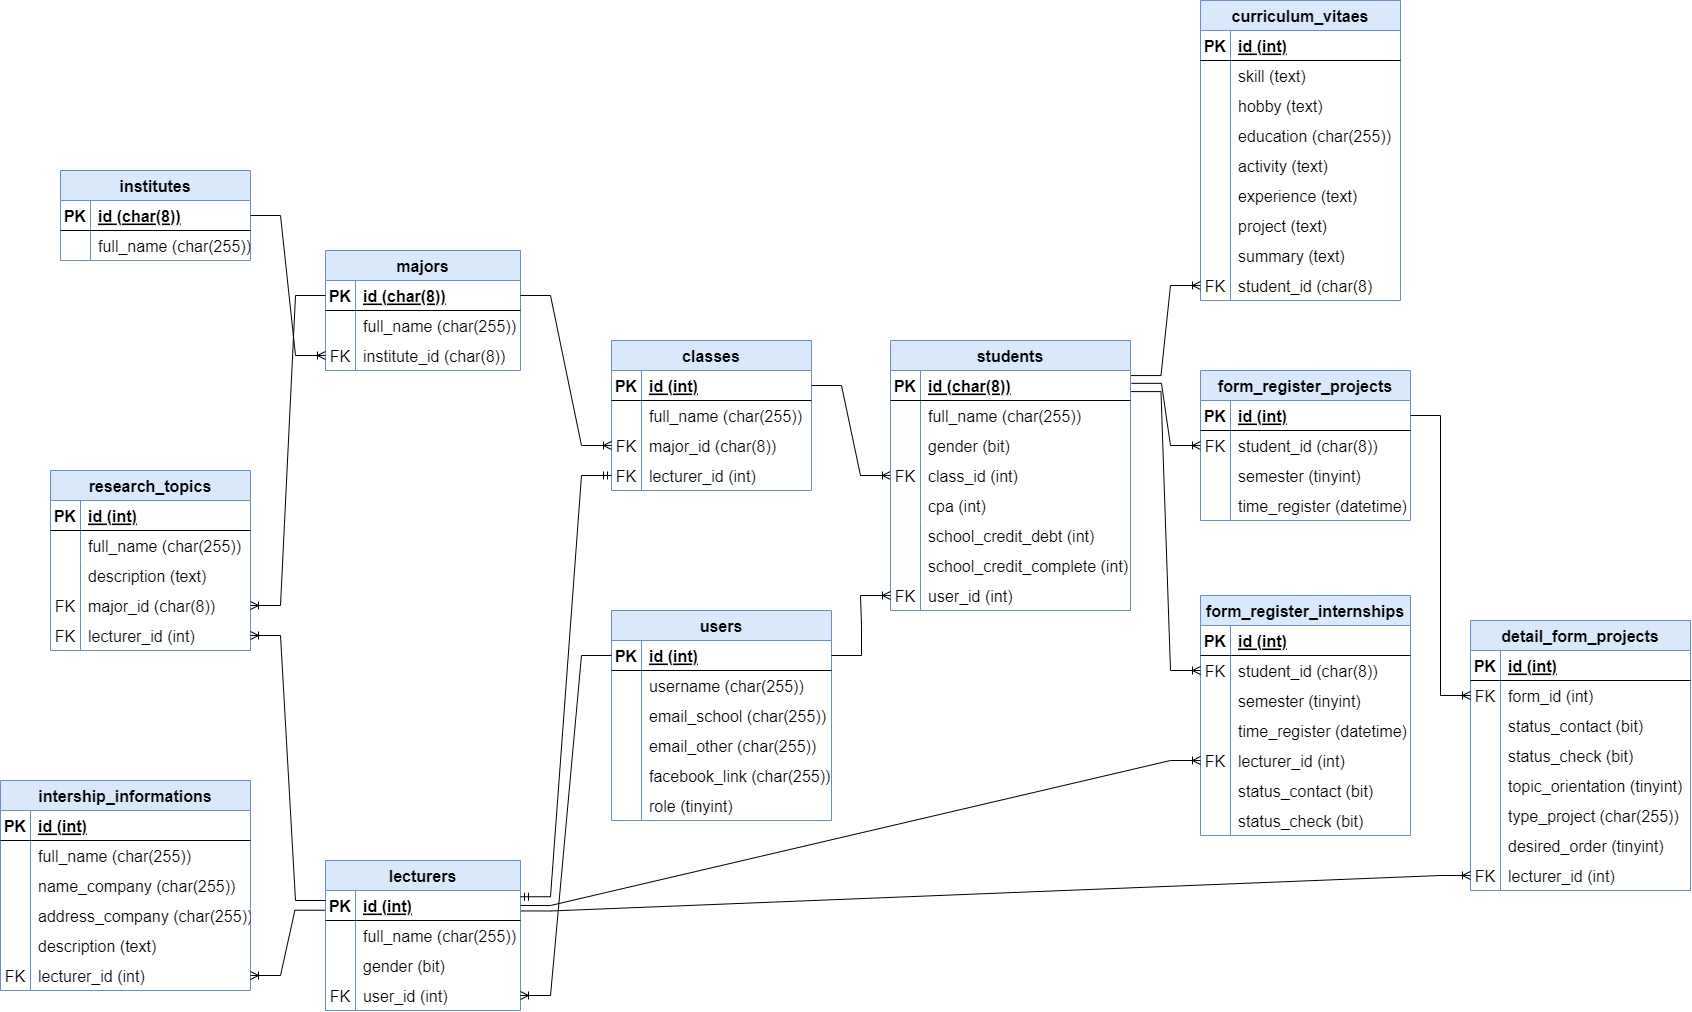
\includegraphics[width=1.5\textwidth]{../drawio/db_sv11.png}
    \begin{figure}[h]
      \centering
      \caption{Biểu đồ dữ liệu quan hệ}
    \end{figure}
  \end{center}
\end{landscape}
% \input{giao_dien.tex}

\end{document}
